%=========================================================================
% (c) Michal Bidlo, Bohuslav Křena, 2008

\chapter{Úvod}
Hlavným cieľom tejto práce je návrh hardvérových komponentov na riešenie rozsiahlych diferenciálnych rovníc. Diferenciálne rovnice sa väčšinou riešia pomocou numerickej integrácie, a teda s~použitím vhodných numerických metód. Hardvérový komponent využívajúci numerickú integráciu sa nazýva numerický integrátor.

V~kapitole~\ref{NUM_INTEGRACIA} sú predstavené rôzne numerické metódy - Eulerova metóda, metóda Runge-Kutta a Taylorov rad. Najväčšia pozornosť je venovaná metóde Taylorovej rady, ktorá poskytuje vhodný pomer medzi rýchlosťou a presnosťou \cite{KunovskyH}. Bližší popis a práca s~toutou metódou sú uvedené v~kapitole~\ref{SOLUTION_WITH_TAYLOR}. Ukážeme si rozdelenie Taylorovej rady na jednotlivé členy a následne úpravu týchto členov tak, aby bolo možné výpočet čo najviac paralelizovať a optimalizovať. Táto úprava bude realizovaná na obyčajných diferenciálych rovniciach s~operáciou násobenia a delenia. Takto upravené a vytvorené rovnice budú následne použité pri návrhu rôznych typov numerických integrátorov.

Kapitola~\ref{REPREZENTACIA_OPERANDOV} sa zaoberá reprezentáciou operandov v~pevnej a v~pohyblivej rádovej čiarke. Pri použití pohyblivej rádovej čiarky sú uvedené postupy výpočtu znamienka, exponentu a mantisy na jednoduchých matematických operáciách, ako sú sčítanie, odčítanie, násobenie a delenie.

V~kapitole~\ref{NUM_INTEGRATORY} sú predstavené a popísané návrhy jednotlivých integrátorov a popis ich činnosti. Podľa rovníc uvedených v~kapitole~\ref{SOLUTION_WITH_TAYLOR} sú navrhnuté paralelné numerické integrátory s~operáciou násobenia a delenia. Oba integrátory sú navrhnuté v~prevedení pevnej a pohyblivej rádovej čiarky. Vzájomným zapojením navrhnutých numerických integrátorov je možné riešiť rozsiahle diferenciálne rovnice.

Navrhnuté integrátory budú popísane vo VHDL. Podrobnejší popis implementácie obsahuje kapitola \ref{IMPLEMENTACIA}. Integrátory následne otestujeme v prostredí \textit{ModelSim} použitím \textit{tesbanchu}. Takto pripravené integrárory sú implementované na FPGA, a to samostatne a v zapojení do sústavy.

Kapitola \ref{ANALYZA} obsahuje časovú analýzu jednotlivých integrátorov v zapojení do sústavy. Ďalej je analyzovaná presnosť použitej Taylorovej rady s metódami nižšieho rádu, ktoré sú popísane v kapitole \ref{NUM_INTEGRACIA}.




%Operácia delenia je realizovaná pomocou deliacho algoritmu SRT. Bližší popis tohto algoritmu sa nachádza v~bakalárskej práci Simulátor procesora s~operáciou delenia \cite{MatecnyBP}.





\chapter{Numerická integrácia} \label{NUM_INTEGRACIA}
%popis počáteční úlohy, diskretizace, exaktné/numerické riešenie
Diferenciálne rovnice sú matematické rovnice, v~ktorých ako premenné vystupujú derivácie funkcií. Najvyššia derivácia v~rovnici udáva rád rovnice. Rovnice, ktoré obsahujú derivácie len podľa jednej premennej, sa nazývajú obyčajné diferenciálne rovnice (ODR). Rovnice, ktoré obsahujú derivácie podľa viacerých premenných, sú takzvané parciálne diferenciálne rovnice (PDR).
V tejto práci sa budeme zaoberať s diferenciálnymi rovnicami prvého rádu. Tie je možné vyjadriť v tvare: 

\begin{eqnarray}
y'(t) = f(t, y(t)) , \label{pocrovnica}
\end{eqnarray}

kde je potrebné zvoliť hodnotu funkcie v bode $ t = t_0 $, t. j. počiatočnú podmienku
\begin{eqnarray}
y(t_0) = y_0. \label{pocpodmienka}
\end{eqnarray}

Obe rovnice \eqref{pocrovnica} a \eqref{pocpodmienka} tvoria počiatočnú úlohu, taktiež nazývanú ako Couchyova úloha. Budeme uvažovať že funkcia \eqref{pocrovnica} je Lipschitzovsky spojitá a ohraničená, potom Cauchyova úloha má práve jedno riešenie \cite{SatekDisP}. 
Diferenciálnu rovnicu je možné riešiť analyticky alebo použitím numerickej metódy. Pri väčšine praktických úloh je analytické riešenie veľmi zložité, preto sa používa skôr riešenie numerické. Základným princípom numerického riešenia je diskretizácia premenných, keď spojitú veličinu nahradíme postupnosťou diskrétnych bodov. Pri použití dostatočne hustého rozloženia bodov môžeme približne reprezentovať spojitú veličinu. Vzdialenosť medzi dvoma susednými bodmi sa nazýva krok metódy. Numerické metódy pri svojom výpočte používajú niekoľko predchádzajúcich krokov. Podľa počtu týchto krokov rozdeľujeme numerické metódy na metódy jednokrokové a viackrokové. Jednokrokové metódy pri svojom výpočte používajú len jeden predchádzajúci krok, viackrokové metódy využívajú niekoľko predchádzajúcich krokov. Pri numerických metódach je teda potrebné zvoliť počiatočný stav, t. j. počiatočnú podmienku riešenej úlohy. Od nej sa následne počíta hodnota funkcie v ďalšom bode \cite{NumMetody}. 

Hlavnými kritériami pri numerických metódach sú presnosť a rýchlosť. Tie je možné ovplyvniť veľkosťou integračného kroku a rádom integračnej metódy. Pri počítaní numerickými metódami nedostávame teoreticky presné riešenie, ale výsledok konverguje k~správnemu riešeniu, a teda dostávame výsledok s~určitou presnosťou. Výsledná chyba výpočtu je súčet lokálnej a akumulovanej chyby.  Lokálna chyba zahŕňa chybu numerickej metódy a zaokrúhľovaciu chybu, ktorá môže byť spôsobená typom hardvérovej architektúry, ako napríklad použitím pevnej alebo pohyblivej rádovej čiarky, ktoré sú bližšie popísané v~kapitole \ref{REPREZENTACIA_OPERANDOV}. Akumulovaná chyba je súčtom lokálnych chýb, čiže sa počas výpočtu zvyšuje. Chyba v jednom kroku teda ovplyvňuje výsledky krokov nasledujúcich.


\section{Taylorova rada}
Táto numerická metóda je tvorená nekonečným radom, avšak na výpočet sa používa len niekoľko jej členov. Počet použitých členov udáva rád metódy. Čím väčší počet členov použijeme, tým je výsledok presnejší. Počet použitých členov môže byť zadaný fixne, alebo sa môže dynamicky meniť v~závislosti od požadovanej presnosti. Presnosť sa počíta pomocou viacerých najvyšších členov. Po dosiahnutí požadovanej presnosti výpočet končí.
Nekonečnú Taylorovu radu môžeme zapísať:

\begin{eqnarray}
y_{i + 1} = y_{i} + h y'_{i} + \dfrac{h^{2}}{2!}y''_{i} + \dfrac{h^{3}}{3!}y'''_{i} + \dfrac{h^{4}}{4!}y^{(4)}_{i} + \cdots + \dfrac{h^{n}}{n!}y_{i}^{(n)} \, , \label{Taylor}
\end{eqnarray}

kde $ h $ je veľkosť integračného kroku a $ i $ označuje krok diskretizovanej veličiny. Ďalšie popísané metódy sú odvodené od Taylorovej rady.


\section{Eulerova metóda}
Najjednoduchšou jednokrokovou metódou na riešenie počiatočnej (Cauchyho) úlohy je Eulerova metóda. Je to Taylorova metóda 1. rádu, keďže používa len prvé dva členy Taylorovej rady. Je preto rýchla, no menej presná. Zapisuje sa nasledovne:

\begin{eqnarray}
y_{i+1} = y_{i} + hy'_{i} \, .
\end{eqnarray}

Zvolením dostatočne malého integračného kroku $ h $ môžeme zvýšiť jej presnosť. Čím je však krok menší, tým je výpočet pomalší.


\section{Runge-Kutta}
Ďalšou veľmi známou numerickou metódou je Runge-Kutta. Všeobecná schéma tejto metódy má tvar:

\begin{eqnarray}
y_{i+1} & = & y_{i} + \sum^{r}_{j=1} \alpha_{j}k_{j} \\
k_{1} & = & f(x_{i},y_{i}) \nonumber \\
k_{j} & = & f(x_{i} + \lambda_{j}h, y_{i} + \mu_{j}hk_{j-1}) , \quad j=2,\dotsc r \, , \nonumber
\end{eqnarray}

kde $\alpha_{j}, \lambda_{j}$ a $\mu_{j}$ sú vhodne zvolené konštanty a $ r $ určuje rád metódy. Ako je v~uvedených rovnciach vidieť, pri výpočte sa používajú medzivýpočty $ k $, ktorých počet sa rovná rádu metódy.
Najznámejšie a najčastejšie používané varianty sú Runge-Kutta 2. a 4. rádu, ktoré sú popísané nižšie.

\newpage
\subsection{Runge-Kutta 2. rádu} \label{RK2}
Táto metóda je oproti Eulerovej metóde presnejšia, ale pri rovnakej veľkosti integračného kroku vyžaduje viac operácií. Na výpočet používa dva medzivýpočty $ k_{1} $ a $ k_{2} $. Má nasledujúci tvar:

\begin{eqnarray}
y_{i+1} & = & y_{i} + \frac{1}{2}h(k_{1} + k_{2}) \\
k_{1} & = & f(t_{i},y_{i}) \nonumber \\
k_{2} & = & f(t_{i+1}, y_{i} + hk_{1}) \, . \nonumber
\end{eqnarray}


\subsection{Runge-Kutta 4. rádu} \label{RK4}
Runge-Kutta 4. rádu je najpoužívanejší tvar tejto metódy. Môžeme ho zapísať nasledovne:

\begin{eqnarray}
y_{i+1} & = & y_{i} + \frac{1}{6}h(k_{1} + 2k_{2} + 2k_{3} + k_{4}) \\
k_{1} & = & f(t_{i},y_{i}) \nonumber \\
k_{2} & = & f(t_{i+1} + \frac{1}{2}h, y_{i} + \frac{1}{2}hk_{1}) \nonumber \\
k_{3} & = & f(t_{i+1} + \frac{1}{2}h, y_{i} + \frac{1}{2}hk_{2}) \nonumber \\
k_{4} & = & f(t_{i+1} + h, y_{i} + hk_{3}) \, . \nonumber
\end{eqnarray}

Napriek tomu, že sú pri výpočte použité štyri medzivýpočty, má táto metóda dobrý pomer rýchlosti a presnosti.


\chapter{Riešenie diferenciálnych rovníc Taylorovou radou} \label{SOLUTION_WITH_TAYLOR}
Na riešenie diferenciálnych rovníc je možné upraviť základný tvar Taylorovej rady \eqref{Taylor} tak, aby sa dali jednotlivé operácie vykonávať paralelne. Prevod jednoduchej obyčajnej diferenciálnej rovnice je prevzatý z~\cite{MatecnyBP}. Ďalšími možnými zdrojmi sú \cite{OpalkaDP}, \cite{KrausDisP}. V ďalších častiach tejto práce budeme používať označenie \textit{N} pre použitý rád Taylorovej metódy t. j. maximálny počet použitých členov. Symbol \textit{n} bude označovať akruálne spracovávaný člen Taylorovej rady. \\

Majme zadanú konkrétnu obyčajnú diferenciálnu rovnicu (počiatočnú úlohu):
\begin{eqnarray}
y' = y \, , \quad y(0) = y_{0}. \, \label{jednoducha_rovnica}
\end{eqnarray}

Z~tohoto vzťahu vyplýva, že:
\begin{eqnarray}
y = y' = y'' = y''' = y^{(4)} =\cdots = y^{(N)} .
\end{eqnarray}

Po dosadení do Taylorovej rady \eqref{Taylor} získame:
\begin{eqnarray}
y_{i + 1} = y_{i} + h y_{i} + \dfrac{h^{2}}{2!}y_{i} + \dfrac{h^{3}}{3!}y_{i} + \dfrac{h^{4}}{4!}y_{i} + \cdots + \dfrac{h^{N}}{N!}y_{i} .
\end{eqnarray}


To je možné prepísať na:
\begin{eqnarray}
y_{i + 1} = y_{i} + DY1_{i} + DY2_{i} + DY3_{i} + DY4_{i} + \cdots + DY(N)_{i} \, , \label{TaylorDYcleny}
\end{eqnarray}

kde je význam jednotlivých členov nasledujúci:
\begin{eqnarray}
DY1_{i} & = & h y_{i} \label{DY_cleny} \\
DY2_{i} = \dfrac{h^{2}}{2!}y_{i} & = & \dfrac{h}{2} DY1_{i} \nonumber \\
DY3_{i} = \dfrac{h^{3}}{3!}y_{i} & = & \dfrac{h}{3} DY2_{i} \nonumber \\
DY4_{i} = \dfrac{h^{4}}{4!}y_{i} & = & \dfrac{h}{4} DY3_{i} \nonumber \\
& \vdots & \nonumber
%DY(N)_{i} =  \dfrac{h^{n}}{n!}y_{i} & = & \dfrac{h}{n} DY(N-1)_{i} \nonumber
\end{eqnarray}

Všeobecný zápis:
\begin{equation}
DY(n)_{i} =  \dfrac{h^{n}}{n!}y_{i} = \dfrac{h}{n} DY(n-1)_{i} \nonumber
\end{equation}

Na základe týchto vzťahov je možné riešiť jednoduché diferenciálne rovnice, ako to je uvedené napríklad v \cite{OpalkaBP} alebo v \cite{KrausDisP}.
Zo vzťahov taktiež vyplýva, že každý ďalší člen Taylorovej rady je počítaný z~predchádzajúceho člena, čo vedie k~zefektívneniu výpočtu, a to najmä pri vyšších deriváciách, v ktorých je výpočet častokrát zložitý. Podobným postupom je možné upraviť diferenciálne rovnice, ktoré obsahujú operáciu násobenia alebo delenia, a tiež tak zvýšiť efektivitu výpočtu týchto výpočtovo náročnejších operácií. 


\section{Riešenie diferenciálnej rovnice s~operáciou násobenia}
Všeobecný zápis pre diferenciálnu rovnicu s operáciou násobenia je nasledujúci:
\begin{eqnarray}
y' & = & qr \, , \quad y(0) = y_{0} . \label{dif_nasobenie}
\end{eqnarray}

Pre výpočet každej premennej v rovnici je potrebné použiť Taylorovu radu v tvare \eqref{TaylorDYcleny}. Jednotlivé Taylorove rady vyzerajú nasledovne:
\begin{eqnarray}
y_{i + 1} & = & y_{i} + DY1_{i} + DY2_{i} + DY3_{i} + DY4_{i} + \cdots + DY(N)_{i}\\
q_{i+1} & = & q_i + DQ1_i + DQ2_i + DQ3_i + DQ4_i + \cdots + DQ(N)_i\\
r_{i+1} & = & r_i + DR1_i + DR2_i + DR3_i + DR4_i + \cdots + DR(N)_i .
\end{eqnarray}


Spočítame jednotlivé derivácie rovnice \eqref{dif_nasobenie}:
\begin{eqnarray}
y' & = & qr \nonumber \\
y'' & = & q'r + qr' \nonumber \\
y''' & = & q''r + 2q'r' + qr'' \nonumber \\
y^{(4)} & = & q'''r + 3q''r'+ 3q'r'' + qr''' \nonumber \\
 & \vdots \nonumber &
\end{eqnarray}


Ako je vidieť, derivácie vytvárajú Pascalov trojuholník a môžeme ich všeobecne zapísať ako
\begin{equation}
y^{(n+1)} = \sum_{k=0}^n \binom{n}{k} q^{(n-k)} r^{(k)} . \nonumber
\end{equation}
\bigskip

Z derivácií odvodíme jednotlivé členy Taylorovej rady \eqref{Taylor}, ktoré majú nasledujúci význam:
\begin{eqnarray}
\dfrac{DY1_{i}}{h} & = & DQ0_i DR0_i \\
\dfrac{DY2_{i}}{\frac{h^{2}}{2!}} & = & \dfrac{DQ1_i}{h} DR0_i + DQ0_i \dfrac{DR1_i}{h} \nonumber \\
\dfrac{DY3_{i}}{\frac{h^{3}}{3!}} & = & \dfrac{DQ2_i}{\frac{h^{2}}{2!}} DR0_i + 2 \dfrac{DQ1_i}{h} \dfrac{DR1_i}{h} + DQ0_i \dfrac{DR2_i}{\frac{h^{2}}{2!}} \nonumber \\
\dfrac{DY4_{i}}{\frac{h^{4}}{4!}} & = & \dfrac{DQ3_i}{\frac{h^{3}}{3!}} DR0_i + 3 \dfrac{DQ2_i}{\frac{h^{2}}{2!}} \dfrac{DR1_i}{h} + 3 \dfrac{DQ1_i}{h} \dfrac{DR2_i}{\frac{h^{2}}{2!}} + DQ0_i \dfrac{DR3_i}{\frac{h^{3}}{3!}} \nonumber \\
& \vdots \nonumber & 
\end{eqnarray}



Po úprave dostaneme konečný tvar jednotlivých členov:
\begin{eqnarray}
DY1_{i} & = & hq_{i}r_{i} \label{DY1_cleny_nasobenia} \\
DY2_{i} & = & \frac{h}{2} (DQ1_{i}DR0_{i} + DQ0_{i}DR1_{i}) \label{DY2_cleny_nasobenia} \\
DY3_{i} & = & \frac{h}{3} (DQ2_{i}DR0_{i} + DQ1_{i}DR1_{i} + DQ0_{i}DR2_{i}) \label{DY3_cleny_nasobenia} \\
DY4_{i} & = & \frac{h}{4} (DQ3_{i}DR0_{i} + DQ2_{i}DR1_{i} + DQ1_{i}DR2_{i} + DQ0_{i}DR3_{i}) \label{DY4_cleny_nasobenia} \\
& \vdots \nonumber &
\end{eqnarray}

Všeobecný zápis:
\begin{equation}
DY(n)_{i} = \dfrac{h}{n} \cdot \left( \sum_{k=1}^n DQ(n-k)_{i} \cdot DR(k-1)_{i} \right) . \label{suma_mul}
\end{equation}

Uvedený prevod vychádza z práce \cite{ZavadaBP}. Jednotlivé rovnice členov Taylorovej rady budú slúžiť pri návrhu a implementácii násobiacich integrátorov.


\section{Riešenie diferenciálnej rovnice s~operáciou delenia}
Podobne ako v~predchádzajúcom prípade, zapíšme diferenciálnu rovnicu s~operáciou delenia nasledovne:
\begin{eqnarray}
y' & = & \dfrac{u}{v} \, , \quad y(0) = y_{0} . \label{dif_delenie}
\end{eqnarray}



Jednotlivé Taylorove rady pre premenné v rovnici vyzerajú nasledovne:
\begin{eqnarray}
y_{i + 1} & = & y_{i} + DY1_{i} + DY2_{i} + DY3_{i} + DY4_{i} + \cdots + DY(N)_{i}\\
u_{i+1} & = & u_i + DU1_i + DU2_i + DU3_i + DU4_i + \cdots + DU(N)_i\\
v_{i+1} & = & v_i + DV1_i + DV2_i + DV3_i + DV4_i + \cdots + DV(N)_i .
\end{eqnarray}



Ďalšie derivácie rovnice \eqref{dif_delenie} sú:
\begin{eqnarray}
y'' = \dfrac{u'v - uv'}{v^{2}} & = & \dfrac{1}{v} (u' - y'v') \label{derivacie_delenie} \\
y''' = \left( \dfrac{1}{v} (u' - y'v') \right)' & = & \dfrac{1}{v} (u'' - 2y''v' - y'v'') \nonumber \\
y^{(4)} = \left( \dfrac{1}{v} (u'' - 2y''v' - y'v') \right)' & = & \dfrac{1}{v} (u''' - 3y'''v' - 3y''v'' - y'v''') \nonumber \\
 & \vdots \nonumber &
\end{eqnarray}

Aj tu je vidieť, že jednotlivé derivácie tvoria Pascalov trojuholník. Všeobecný zápis je nasledovný:
\begin{equation}
y^{(n+1)} = \dfrac{1}{v} \left( u^{(n)} - \left( \sum_{k=1}^n \binom{n}{k} y^{(n-k+1)} v^{(k)} \right) \right) . \nonumber
\end{equation}
\bigskip

Po dosadení jednotlivých členov $ DV(n)_{i} $ a $ DU(n)_{i} $ do derivácií \eqref{derivacie_delenie} dostaneme:
\begin{eqnarray}
\dfrac{DY1_{i}}{h} & = & \frac{1}{v} u~\\
\dfrac{DY2_{i}}{\frac{h^{2}}{2!}} & = & \dfrac{1}{v} ( \dfrac{DU1_{i}}{h} - \dfrac{DY1_{i}}{h}\dfrac{DV1_{i}}{h} ) \nonumber \\
\dfrac{DY3_{i}}{\frac{h^{3}}{3!}} & = & \dfrac{1}{v} 
( \dfrac{DU2_{i}}{\frac{h^{2}}{2!}} - 
2\dfrac{DY2_{i}}{\frac{h^{2}}{2!}} \dfrac{DV1_{i}}{h} - 
\dfrac{DY1_{i}}{h} \dfrac{DV2_{i}}{\frac{h^{2}}{2!}} ) \nonumber \\
\dfrac{DY4_{i}}{\frac{h^{4}}{4!}} & = & \dfrac{1}{v} 
( \dfrac{DU3_{i}}{\frac{h^{3}}{3!}} - 
3\dfrac{DY3_{i}}{\frac{h^{3}}{3!}} \dfrac{DV1_{i}}{h} - 
3\dfrac{DY2_{i}}{\frac{h^{2}}{2!}} \dfrac{DV2_{i}}{\frac{h^{2}}{2!}} -
\dfrac{DY1_{i}}{h} \dfrac{DV3_{i}}{\frac{h^{3}}{3!}} ) \nonumber \\
& \vdots \nonumber & 
\end{eqnarray}


Po úprave majú jednotlivé členy Taylorovej rady nasledovný tvar:
\begin{eqnarray}
DY1_{i} & = & \frac{1}{v_{i}} (hu_{i}) \label{DY1_cleny_delenia} \\
DY2_{i} & = & \dfrac{1}{2v_{i}} (DU1_{i}h - DY1_{i}DV1_{i}) \label{DY2_cleny_delenia} \\
DY3_{i} & = & \dfrac{1}{3v_{i}} ( DU2_{i}h - 2DY2_{i}DV1_{i} - DY1_{i}DV2_{i} ) \label{DY3_cleny_delenia} \\
DY4_{i} & = & \dfrac{1}{4v_{i}} ( DU3_{i}h - 3DY3_{i}DV1_{i} - 2DY2_{i}DV2_{i} - DY1_{i}DV3_{i} ) \label{DY4_cleny_delenia} \\ 
& \vdots \nonumber & 
\end{eqnarray}

Všeobecný zápis:
\begin{equation}
DY(n)_{i} = \dfrac{1}{n DV0_{i}} \cdot \left( DU(n-1)_{i} \cdot h - \left( \sum_{k=1}^{n-1} (n-k) \cdot DY(n-k)_{i} \cdot DV(k)_{i} \right) \right)  .\label{suma_div}
\end{equation}
\bigskip

Vyjadrenie jednotlivých členov Taylorovej rady vychádza z~bakalárskej práce~\cite{MatecnyBP}. Takto upravené členy sú následne použité na návrh jednotlivých typov integrátorov popísaných v~kapitole~\ref{NUM_INTEGRATORY}.



\chapter{Reprezentácia operandov} \label{REPREZENTACIA_OPERANDOV}
Čísla vo výpočtových systémoch sú reprezentované rôznymi spôsobmi v~závislosti od zvolenej aritmetiky. Najpoužívanejšie reprezentácie čísiel sú zapísané v~pevnej a v~pohyblivej rádovej čiarke (ang. fixed point (FX) a floating point (FP)). Obe aritmetiky sú popísané v nasledujúcich podkapitolách. Informácie v~tejto kapitole sú čerpané z~\cite{FXOnline}, \cite{FPOnline}, \cite{KrausDisP}, \cite{inpFP}, \cite{inpRepDat}.


\section{Pevná rádová čiarka}
Pri počítaní v~pevnej rádovej čiarke sú čísla reprezentované na $ k $ bitoch v~tvare $ n.m $, kde prvých $ n $ bitov tvorí časť čísla pred desatinnou čiarkou a zostávajúcich $ m $ bitov tvorí číslo za desatinnou čiarkou. Pozícia desatinnej čiarky je dopredu známa. V~závislosti od jej pozície sa používajú rôzne formáty pevnej rádovej čiarky. Tie najpoužívanejšie sú znázornené na obrázku~\ref{formatfixpoint}. \\
Obrázok \ref{formatfixpointa} zobrazuje aritmetiku s nulovým počtom bitov za desatinnou čiarkou, a teda ide o celočíselnú aritmetiku na $ n $ bitoch. Vedľajší obrázok \ref{formatfixpointb} zobrazuje aritmetiku s $ n $ bitmi pred desatinnou čiarkou a s $ m $ bitmi za desatinou čiarkou. Ďalšia časť obrázku \ref{formatfixpointc} je opakom \ref{formatfixpointa}, kde je číslo reprezentované len za desatinou čiarkou na $ m $ bitoch. Posledný obrázok \ref{formatfixpointd} je podobný ako \ref{formatfixpointc}, no má pridaný znamienkový bit $ S $.
V tejto práci budeme používať FX aritmetiku v tvare \ref{formatfixpointb} s pridaným znamienkovým bitom na pozícii MSB (most significant bit).

%\bigskip
%\begin{figure}[h]
%\centering
%\scalebox{0.9}{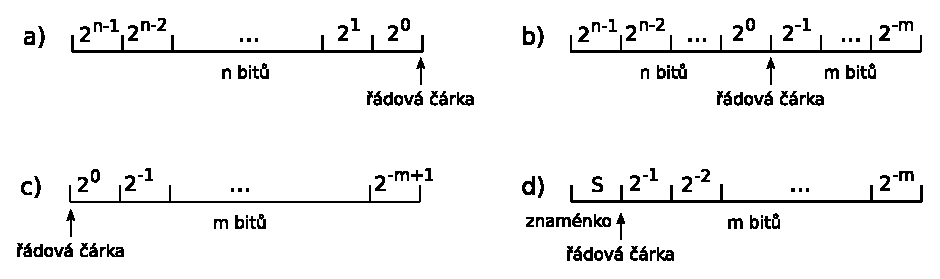
\includegraphics{obrazky/pevna_rad_carka.eps}}
%\caption{Rôzne formáty fixed point aritmetiky \cite{KrausDisP}}
%\label{formatfixpoint}
%\end{figure}
%\bigskip

\begin{figure}[h]
\centering
\subfloat{\label{formatfixpointa} 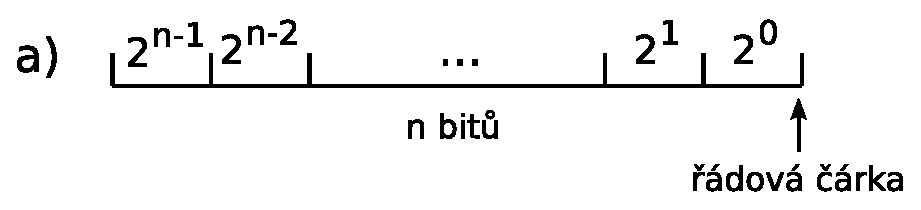
\includegraphics[width=0.44\linewidth]{obrazky/pevna_rad_carkaa.eps}} \hspace{0.6cm}
\subfloat{\label{formatfixpointb} 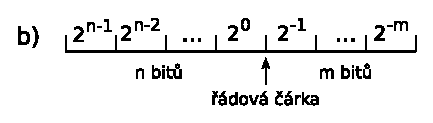
\includegraphics[width=0.405\linewidth]{obrazky/pevna_rad_carkab.eps}} \\ \bigskip
\subfloat{\label{formatfixpointc} 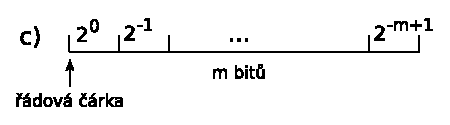
\includegraphics[width=0.405\linewidth]{obrazky/pevna_rad_carkac.eps}} \hspace{1.2cm}
\subfloat{\label{formatfixpointd} 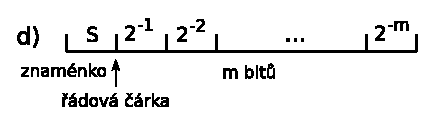
\includegraphics[width=0.405\linewidth]{obrazky/pevna_rad_carkad.eps}}
\caption{Rôzne formáty fixed point aritmetiky \cite{KrausDisP}}
\label{formatfixpoint}
\end{figure}
\bigskip

%Môžeme si všimnúť, že čísla uložené vo FX sú rovnomerne rozložené na časovej osi.
Vo fixed point aritmetike sa používajú rôzne kódy, napr. priamy kód, doplnkový kód či inverzný kód. V~nasledujúcich kapitolách a pri návrhu integrátorov v~pevnej rádovej čiarke budeme používať doplnkový kód. 

\newpage
\section{Pohyblivá rádová čiarka}
Čísla uložené v~pohyblivej rádovej čiarke sú tvorené exponentom a mantisou. Všeobecný tvar na získanie hodnoty uloženej vo FP je nasledujúci:

\begin{eqnarray}
X = B^{E}\cdot M
\end{eqnarray}

\begin{tabular}{ll}
$ X $ - výsledná hodnota \\
$ B $ - základ sústavy \\
$ E $ - hodnota exponenta \\
$ M $ - mantisa \\
\end{tabular}
\bigskip

Zvýšením počtu bitov v~exponente $ E $ sa zvýši rozsah hodnôt, ktorý je možné reprezentovať, a zvýšením počtu bitov v~mantise $ M $ za zvýši presnosť uložených čísel. Existuje veľa formátov uloženia čísel v~pohyblivej rádovej čiarke. Najpoužívanejší a najrozšírenejší je štandard \textbf{IEEE 754}. Ten definuje vlastný formát uloženia čísel a viaceré formáty s~rôznou presnosťou. Najpoužívanejšie z~nich sú formáty čísel s~jednoduchou (single) a s~dvojitou (double) presnosťou. Čísla s~jednoduchou presnosťou sú uložené na 32 bitoch, kde MSB je znamienkový bit $ S $, ďalších 8 bitov tvorí exponent $ E $ a zvyšných 23 bitov tvorí mantisu $ M $.

\bigskip
\begin{figure}[h]
\centering
\scalebox{0.2}{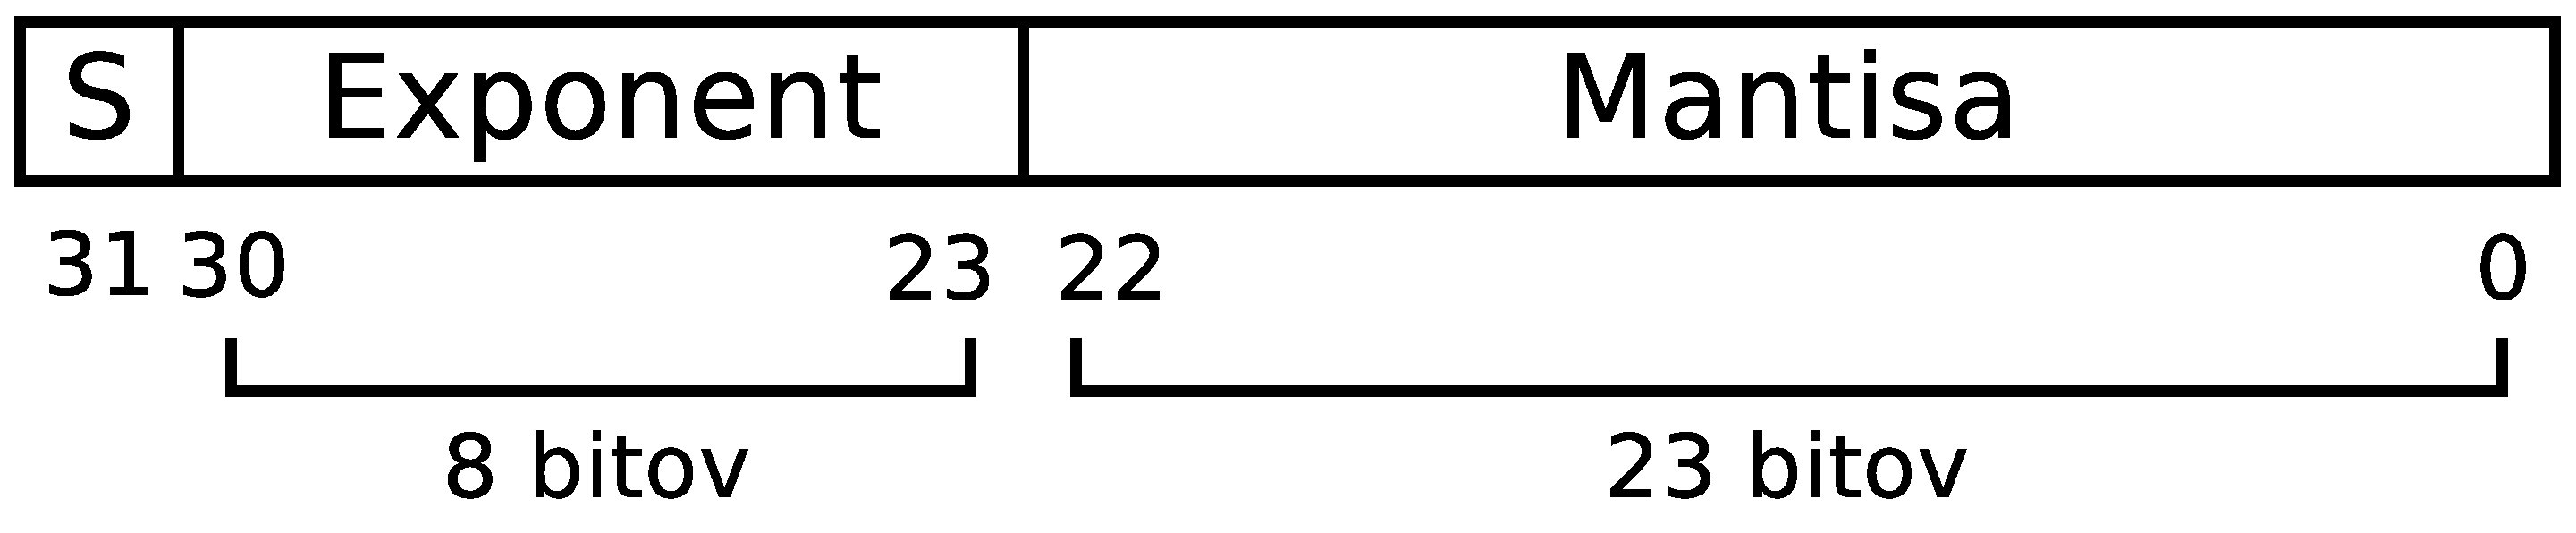
\includegraphics{obrazky/IEEE754_32b.eps}}
\caption{IEEE 754 formát s~jednoduchou presnosťou}
\label{formatFP32}
\end{figure}


Čísla s~dvojitou presnosťou sú uložené v~rovnakom formáte ako čísla s~jednoduchou presnosťou, avšak počet bitov je zvýšený o dvojnásobok. Dvojitá presnoť je teda tvorená 64 bitmi, kde MSB je znamienkový bit $ S $, ďalších 11 bitov tvorí exponent $ E $ a zvyšných 52 bitov tvorí mantisu $ M $.

\bigskip
\begin{figure}[h]
\centering
\scalebox{0.2}{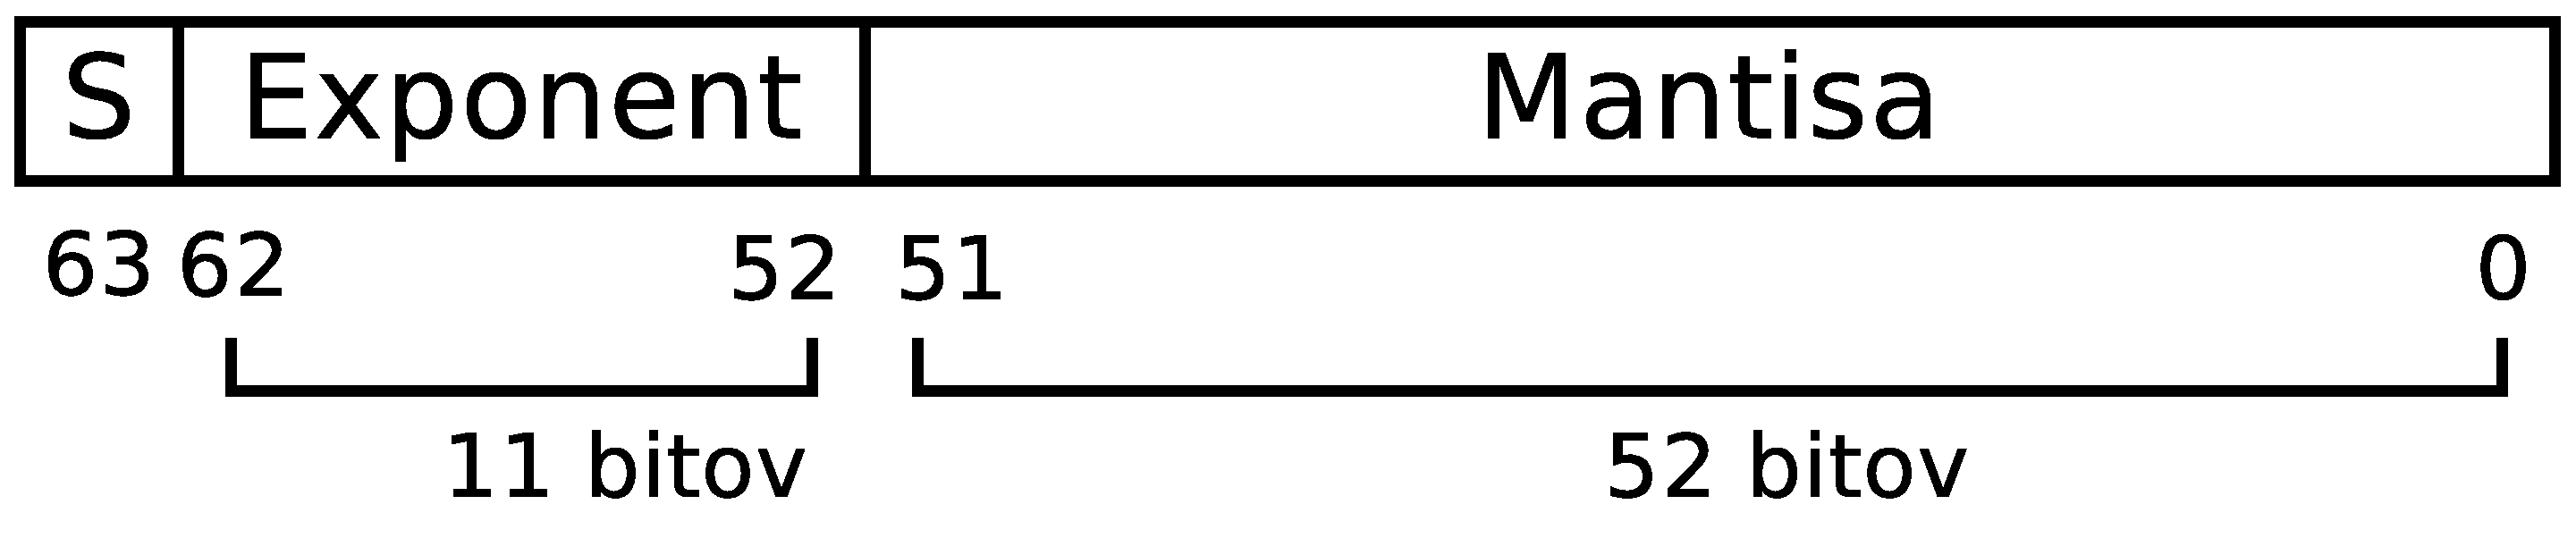
\includegraphics{obrazky/IEEE754_64b.eps}}
\caption{IEEE 754 formát s~dvojitou presnosťou}
\label{formatFP64}
\end{figure}

Znamienko $ S $ nadobúda hodnotu 0, čo znamená kladné číslo; alebo hodnotu 1, čo znamená záporné číslo. Exponent je uložený v~kóde s~nepárnym posunutím o~hodnotu BIAS. Táto hodnota je zvolená tak, aby bol uložený exponent vždy kladný. Pri jednoduchej presnosti má teda BIAS hodnotu 127 a pri dvojitej presnosti hodnotu 2047.
\newpage
Hodnota mantisy je uložená v~priamom kóde bez znamienka, znížená o~hodnotu 1, keďže je tu použitá tzv. normalizácia. Mantisa je normalizovaná do tvaru $ 1.M $, kde sa jednotka neukladá -- je skrytá, čím sa ušetrí jeden bit. Hodnotu takto uloženého čísla získame zo vzťahu:

\begin{eqnarray}
X_{754} = -1^{S}\cdot 2^{E-BIAS}\cdot (1,M)
\end{eqnarray}

\begin{tabular}{ll}
$ X_{754} $ - výsledná hodnota \\
$ BIAS $ - 127 alebo 2047 \\
$ E $ - hodnota exponentu \\
$ M $ - mantisa \\
\end{tabular}
\bigskip

Štandard IEEE 754 definuje aj špeciálne hodnoty ako kladnú/zápornú nulu, kladné/záporné nekonečno, či hodnotu NaN (not a number). Tieto hodnoty sú uvedené v~tabuľke~\ref{standard_IEEE754}.
Hodnota mantisy v~normalizovanom tvare je v~intervale $ <1,0; 2,0) $. Ak tomu tak nie je, ide o~tzv. denormalizované číslo, a hodnota exponenta je braná ako $ -126 $. Štandard IEEE 754 definuje aj spôsob vykonávania základných matematických operácií, ktoré sú popísané v~sekciách \ref{PlusMinusFP} a \ref{MulDivFP}.

\bigskip
\begin{table}[h]
\centering
\begin{tabular}{|l|l|l|l|}
\hline
\rowcolor[HTML]{68CBD0} 
S~(znamienko) & E (exponent) & M (mantisa)       & význam                    \\ \hline
0/1           & 00000000     & nulová hodnota    & +/- 0                     \\ \hline
0/1           & 00000000     & nenulová hodnota  & +/- denormalizované číslo \\ \hline
0/1           & 1 - 254      & ľubovoľná hodnota & +/- FP číslo              \\ \hline
0/1           & 11111111     & nulová hodnota    & +/- $ \infty  $           \\ \hline
0/1           & 11111111     & nenulová hodnota  & NaN                       \\ \hline
\end{tabular}
\caption{Štandard IEEE 754 \cite{FPOnline}}
\label{standard_IEEE754}
\end{table}

\newpage
\subsection{Súčet a rozdiel} \label{PlusMinusFP}
Súčet a rozdiel v~pohyblivej rádovej čiarke sa počíta podľa vzorcov
\begin{eqnarray}
X + Y = (M_{X}\cdot 2^{E_{X} - E_{Y}} + M_{Y})\cdot 2^{E_{Y}} \text{, kde} \quad E_{X} \leq E_{Y} \\
X - Y = (M_{X}\cdot 2^{E_{X} - E_{Y}} - M_{Y})\cdot 2^{E_{Y}} \text{, kde} \quad E_{X} \leq E_{Y} .
\end{eqnarray}

Postup výpočtu operácie súčtu alebo rozdielu v~pohyblivej rádovej čiarke podľa štandardu IEEE 754 (\cite{FPOnline_operacie}, \cite{CamborBP}) je nasledovný:

\begin{enumerate}  
\item Na začiatku výpočtu sa obe čísla skontrolujú na výskyt špeciálnych hodnôt z~tabuľky~\ref{standard_IEEE754}. Ak ide o~špeciálne číslo, výsledok sa určí podľa tabuľky~\ref{special_plus}. Inak sa pokračuje bodom 2.

\item Vykoná sa porovnanie exponentov. Ak sú exponenty rozdielne, mantisu menšieho čísla posunieme o~rozdiel exponentov doprava. Tým docielime rovnosť oboch exponentov. Pri posune je dôležité, aby sme nezabudli na jednotku, ktorá je skrytá kvôli normalizácii. Posun sa vykonáva spolu s~toutou jednotkou. 

\item Následne sa porovnajú znamienka a podľa výsledku sa vykoná súčet alebo rozdiel mantisy väčšieho čísla a posunutej mantisy. Ak došlo k~pretečeniu, mantisa výsledku sa posunie o~jeden bit doprava a hodnota exponentu sa zvýši. Aby bolo možné pretečenie detekovať, je potrebné vykonávať sčítanie alebo odčítanie mantís na sčítačke o~jeden bit väčšej než je veľkosť mantisy (veľkosťou mantisy sa tu myslí počet bitov potrebných na uloženie mantisy aj so skrytou 1, čiže $ |1.M| + 1 $).

\item Ak je to potrebné, vykoná sa normalizácia. Mantisa sa posunie o~potrebný počet bitov doprava, resp. doľava, tak, aby bola v~tvare $ 1.M $. Exponent sa zvýši, resp. zníži o~daný počet bitov.

\item Na koniec výpočtu sa skontroluje hodnota exponentu. Ak je hodnota maximálna, došlo k~pretečeniu výsledku. Ten sa nastaví podľa znamienka na kladné alebo záporné nekonečno. V~opačnom prípade, ak je hodnota exponentu minimálna (nulová), došlo k~podtečeniu, a výsledok je nastavený podľa znamienka na kladnú alebo zápornú nulu.
\end{enumerate}


\begin{table}[h]
\centering
\begin{tabular}{|l|l|l|}
\hline
\rowcolor[HTML]{68CBD0} 
Hodnota operandu 1 & Hodnota operandu 2 & Výsledok sčítania \\ \hline
FP číslo           & +/- $ \infty $     & +/- $ \infty $    \\ \hline
+/- $ \infty $     & +/- $ \infty $     & +/- $ \infty $    \\ \hline
+ $ \infty $       & - $ \infty $       & NaN               \\ \hline
NaN                & ľubovoľná hodnota  & NaN               \\ \hline
\end{tabular}
\caption{Výsledok operácie sčítania so špeciálnymi hodnotami}
\label{special_plus}
\end{table}

\newpage
\subsection{Násobenie a delenie} \label{MulDivFP}
Násobenie a delenie v~pohyblivej rádovej čiarke sa počíta nasledovne:

\begin{eqnarray}
X \times Y = (M_{X} \cdot M_{Y})\cdot 2^{E_{X} + E_{Y}} \\
X \div Y = ({M_{X}} \div {M_{Y}})\cdot 2^{E_{X} - E_{Y}} .
\end{eqnarray}

Postup výpočtu operácií násobenia a delenia podľa štandardu IEEE 754 (\cite{FPOnline_operacie}, \cite{CamborBP}) je nasledovný:

\begin{enumerate}  
\item Rovnako ako pri sčítaní, aj teraz sa na začiatku výpočtu skontroluje výskyt špeciálnych hodnôt oboch čísel podľa tabuľky~\ref{standard_IEEE754}. Ak ide o~špeciálne číslo, výsledok sa určí podľa tabuľky~\ref{special_nasobenie} alebo \ref{special_delenie}. Pri operácii delenia je potrebné kontrolovať nepovolenú operáciu delenie nulou. Pokračuje sa bodom 2.

\item Pri násobení sa hodnota exponentu vypočíta ako súčet exponentov, od ktorého sa odpočíta hodnota \textit{BIAS}. Pri operácii delenia sa hodnota exponentu vypočíta ako rozdiel exponentov, ku ktorému je pripočítaná hodnota \textit{BIAS}.

\item Výsledná mantisa sa rovná súčinu, resp. podielu mantís. Pri násobení je potrebné použiť násobičku, ktorej bitová šírka sa rovná dvojnásobku počtu bitov mantisy $ 1.M $. Ak dôjde k~pretečeniu alebo k~podtečeniu mantisy, vykoná sa posun mantisy doprava, resp. doľava, a hodnota exponentu sa zvýši, resp. zníži.

\item Pokiaľ je to potrebné, prebehne normalizácia.

\item Na konci výpočtu sa skontroluje hodnota exponentu. Postupuje sa rovnako ako pri operácii súčtu: ak je hodnota exponentu maximálna, nastaví sa podľa znamienka na kladné alebo záporné nekonečno. V~opačnom prípade, ak je hodnota exponentu minimálna (nulová), výsledok sa nastaví podľa znamienka na kladnú alebo zápornú nulu.
\end{enumerate}


\begin{table}[h]
\centering
\begin{tabular}{|l|l|l|}
\hline
\rowcolor[HTML]{68CBD0} 
Hodnota operandu 1 & Hodnota operandu 2 & Výsledok násobenia \\ \hline
kladné/záporné FP číslo & +/- $ \infty $ & +/- $ \infty $ \\ \hline
nula           & +/- $ \infty $ & NaN \\ \hline
+/- $ \infty $ & +/- $ \infty $ & +/- $ \infty $ \\ \hline
NaN & ľubovoľná hodnota & NaN \\ \hline
\end{tabular}
\caption{Výsledok operácie násobenia so špeciálnymi hodnotami}
\label{special_nasobenie}
\end{table}

\begin{table}[h]
\centering
\begin{tabular}{|l|l|l|}
\hline
\rowcolor[HTML]{68CBD0} 
Hodnota operandu 1 & Hodnota operandu 2 & Výsledok násobenia \\ \hline
kladné/záporné FP číslo & +/- 0 & +/- $ \infty $ \\ \hline
0 & 0 & NaN \\ \hline
\end{tabular}
\caption{Výsledok operácie delenia so špeciálnymi hodnotami}
\label{special_delenie}
\end{table}

\chapter{Numerické integrátory} \label{NUM_INTEGRATORY}
Numerický integrátor je hardvérový komponent, ktorý slúži na výpočet numerickej integrácie. Podľa spôsobu výpočtu a komunikácie medzi komponentmi integrátora sa numerické integrátory delia na

\begin{itemize}
\item sériovo-sériové (sériové) integrátory (sériová komunikácia aj výpočet)
\item sériovo-paralelné integrátory (sériová komunikácia a paralelný výpočet)
\item paralelno-paralelné (paralelné) integrátory (paralelná komunikácia aj výpočet)
\end{itemize}

V tejto práci sa budeme zaoberať paralelnými numerickými integrátormi pre jednoduchosť a rýchlosť ich výpočtu. Ďalej môžeme numerické integrátory rozdeliť na jednovstupové a dvojvstupové. Jednovstupový integrátor vykonáva integráciu vstupnej hodnoty a posiela ju na výstup. Schéma tohoto typu integrátora je znázornená na obrázku \ref{schema_i}, a ako vyplýva z názvu, obsahuje jeden vstup pre vstupnú hodnotu. Ďalej obsahuje jeden vstup pre počiatočnú podmienku a jeden výstup pre výsledok výpočtu. Dvojvstupové integrátory obsahujú jeden vstup pre počiatočnú podmienku, dva vstupy pre prívod operandov a jeden výstup pre výsledok výpočtu. Schéma integrátora je znázornená na obrázku \ref{schema_ndi}.


\begin{figure}[H]
\centering
\subfloat[Schéma jednovstupového integrátora]{\label{schema_i} 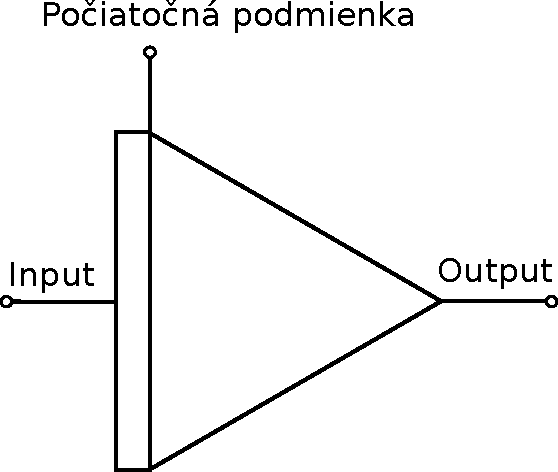
\includegraphics[width=0.4\linewidth]{obrazky/jednoduchy_integrator.pdf}} \hspace{1.0cm}
\subfloat[Schéma dvojvstupového násobiaceho/deliaceho integrátora]{\label{schema_ndi} 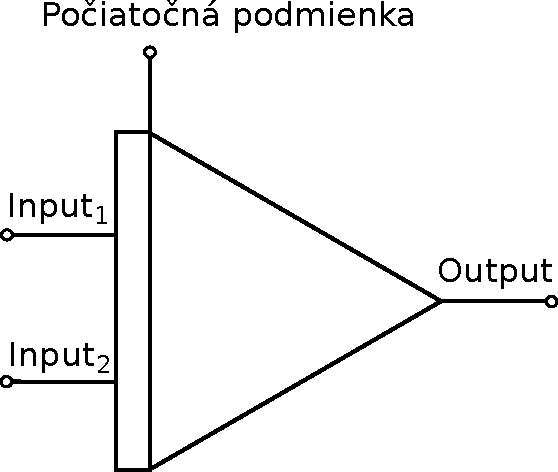
\includegraphics[width=0.4\linewidth]{obrazky/del_nas_integrator.pdf}}
\label{schema_i_ndi}
\caption{Schéma jednovstupového a dvojvstupového integrátora}
\end{figure}

Tieto integrátory rozdeľujeme podľa použitej operácie na násobiace a na deliace integrátory. Násobiaci integrátor vykonáva deriváciu násobenia dvoch vstupných hodnôt. Deliaci integrátor zasa vykonáva deriváciu delenia dvoch vstupných hodnôt. Výsledná hodnota je poslaná na výstup.

V nasledujúcich podkapitolách predstavíme jednotlivé návrhy paralelných násobiacich a paralelných deliacich integrátorov, oba typy v pevnej a v pohyblivej rádovej čiarke. Predstavíme taktiež jednovstupový paralelný integrátor v pevnej a v pohyblivej rádovej čiarke.
\bigskip


\section{Návrh násobiaceho integrátora v~pevnej rádovej čiarke}
Násobiaci integrátor počíta rovnicu \eqref{dif_nasobenie} pomocou \eqref{DY1_cleny_nasobenia} -- \eqref{DY4_cleny_nasobenia}. Na základe týchto rovníc bol vytvorený návrh paralelného násobiaceho integrátora, ktorý je na obrázku~\ref{ppni}. Návrh vychádza z~práce V. Závadu \cite{ZavadaBP} a bol upravený a rozšírený o~počet registrov $ DR(N-1) $ a $ DQ(N-1) $, ktoré slúžia na ukladanie prichádzajúcich členov. Rozšírený bol aj počet registrov pre uloženie kroku $ h $ integračnej metódy a jeho podielov. Počet týchto registrov je o jeden menší ako rád $ ORD $ použitej Taylorovej metódy ($ ORD = N $), keďže pri výpočte sa používajú predchádzajúce členy Taylorovej metódy. Rád metódy je vhodné a potrebné zvoliť vzhľadom na použitú aritmetiku a požadovanú presnosť.

Každý člen $ DY(N-1) $ obsahuje postupné delenie integračného kroku $ h $. Tieto hodnoty sú prepočítané a uložené v~sade registrov $ h $. Pre optimalizáciu a pre ušetrenie miesta však nie je potrebné uložiť všetkých $ N $ hodnôt, stačí uložiť len tie hodnoty, ktorých deliteľom je nepárne číslo. Ostatné hodnoty je možné vypočítať jednoduchým posunom registra doprava, čo je vlastne delenie číslom 2. Je síce potrebné pridať riadiace signály na ovládanie posunu jednotlivých registrov, avšak výsledkom je zníženie počtu registrov $ h $ o~polovicu. Počet operácií potrebných na výpočet sa nezvýši, keďže posun registrov je možné vykonávať v~predstihu a paralelne s~inými operáciami.

\bigskip
\begin{figure}[h]
\centering
\scalebox{0.6}{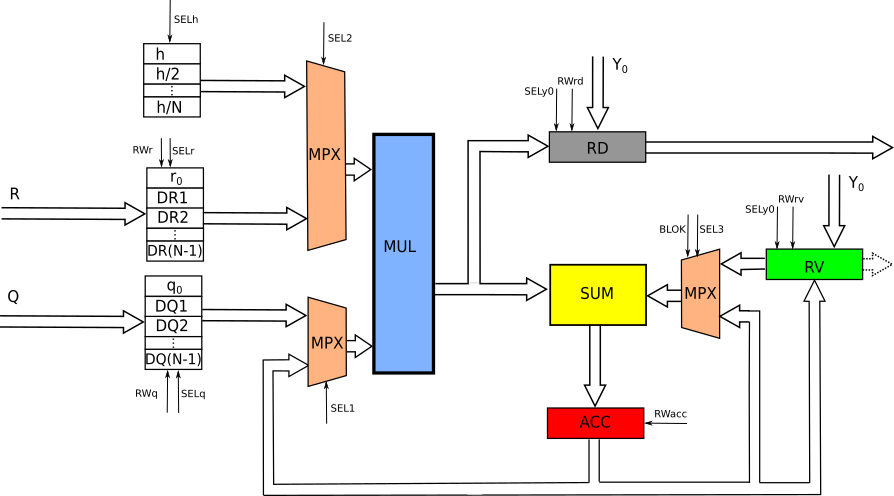
\includegraphics{obrazky/ppni.png}}
\caption{Paralelno-paralelný násobiaci integrátor \cite{ZavadaBP}.}
\label{ppni}
\end{figure}

% Please add the following required packages to your document preamble:
% \usepackage[table,xcdraw]{xcolor}
% If you use beamer only pass "xcolor=table" option, i.e. \documentclass[xcolor=table]{beamer}
\begin{table}[H]
\centering
\begin{tabular}{|
>{\columncolor[HTML]{DAE8FC}}l |l|}
\hline
\multicolumn{1}{|c|}{\cellcolor[HTML]{68CBD0}{\color[HTML]{000000} \textbf{Skratka}}} & \multicolumn{1}{c|}{\cellcolor[HTML]{68CBD0}{\color[HTML]{000000} \textbf{Popis}}} \\ \hline
\textbf{R, Q} & vstupné operandy integrátora \\ \hline
\textbf{Y0} & počiatočná podmienka \\ \hline
\textbf{N} & maximálny rád metódy \\ \hline
\textbf{h, h/2...h/N} & set registrov s integračným krokom metódy a s jeho podielmi \\ \hline
\textbf{r0, DR1, ...DR(N-1)} & set registrov jednotlivých členov vstupného operandu R \\ \hline
\textbf{q0, DQ1, ...DQ(N-1)} & set registrov jednotlivých členov vstupného operandu Q \\ \hline
\textbf{MUL} & paralelná násobička \\ \hline
\textbf{SUM} & paralelná sčítačka \\ \hline
\textbf{ACC} & akumulátor - register na priebežné ukladanie medzivýsledkov \\ \hline
\textbf{RD} & register na uloženie jednotlivých členov Taylorovej rady \\ \hline
\textbf{RV} & register na uloženie celkového výsledku \\ \hline
\textbf{MPX} & multiplexor 2-1 \\ \hline
\textbf{SEL1, SEL2, SEL3} & riadiace signály multiplexorov \\ \hline
\textbf{SELh, SELr, SELq} & riadiace signály registrov \\ \hline
\textbf{SELy0} & riadiaci signál na zápis počiatočnej podmienky \\ \hline
\textbf{RWr, RWq} & povoľovacie signály sád registrov (READ/WRITE) \\ \hline
\textbf{RWrv, RWrd, RWacc} & povoľovacie signály registrov (READ/WRITE) \\ \hline
\textbf{BLOK} & blokový signál multiplexora - na výstupe 0 \\ \hline
\end{tabular}
\caption{Význam skratiek použitých v obrázku \ref{ppni}.}
\label{my-label}
\end{table}

Na začiatku výpočtu sú pomocou signálu \textit{RESET} vynulované všetky registre a nastavia sa potrebné signály na multiplexoroch \textit{MPX}. Následne je do registrov \textit{RV} a \textit{RD} nahraná počiatočná podmienka, do registra \textit{h} je nahraný integračný krok metódy a do registrov \textit{h/i, i=2,3..N} sú nahrané prepočítané hodnoty podielov. Povoľovacím signálom \textit{EN} sa spustí výpočet. Ako prvé sa do registrov uložia vstupné hodnoty \textit{R} a \textit{Q}. Na začiatku každého cyklu výpočtu sú vstupné hodnoty ukladané postupne do ďalších registrov. Po uložení sa začne samotný výpočet. Hodnota aktuálne počítaného člena Taylorovej rady sa postupne ukladá do registra \textit{RD} a odtiaľ je privedená na výstup integrátora.
Do registra \textit{RV} je ukladaný súčet jednotlivých členov Taylorovej rady - čiže celkový výsledok derivácie vstupných hodnôt. Táto hodnota nás bude zaujímať napríklad vtedy, keď je integrátor "posledný" v zapojení, čiže jeho výstup nie je nikam pripojený, a teda nie je potrebné použiť hodnoty jednotlivých členov.


\section{Návrh deliaceho integrátora v~pevnej rádovej čiarke}
Tento integrátor počíta rovnicu \eqref{dif_delenie} pomocou členov \eqref{DY1_cleny_delenia} - \eqref{DY4_cleny_delenia}. Podobne ako pri násobiacom integrátore bol z~týchto rovníc vytvorený návrh paralelného deliaceho integrátora. Návrh vychádza z bakalárskej práce \cite{MatecnyBP} a bol upravený podobne ako predošlý násobiaci integrátor pomocou zvýšenia počtu registrov $ DU(N-1) $ a $ DV(N-1) $. Taktiež sa zvýšil počet registrov $ DY(N-1) $, ktoré slúžia na uloženie jednotlivých členov Taylorovej rady, keďže je na výpočet nasledujúceho člena použitý predchádzajúci člen. Set týchto registrov okrem hodnôt $ DY(N-1) $ obsahuje register na uloženie kroku $ h $ integračnej metódy. Deliaci integrátor, na rozdiel od násobiaceho integrátora, nepotrebuje počas výpočtu hodnoty podielov kroku numerickej metódy, a teda stačí uložiť len jednu hodnotu $ h $. Deliaci integrátor však používa set registrov, ktorý obsahuje hodnoty $ 1/N $. Podobne je možné ako pri násobiacom integrátore, tak aj v deliacom integrátore je možné zmenšiť počet týchto registrov na polovicu s~využitím aritmetického posunu (operácia \textit{shift}). Register \textit{count} obsahuje \textit{counter}, ktorý sa postupne inkrementuje v každom cykle výpočtu, a s~ktorým sa násobí hodnota $ DY(N-1) $. Vyplýva to z rovníc \eqref{DY1_cleny_delenia} - \eqref{DY4_cleny_delenia} a \eqref{suma_div}, kde sa pri výpočte každého člena Taylorovej rady hodnota $ DY(N - k) $ násobí hodnotou $ N - k $. Výsledná vynásobená hodnota je uložená opätovne do daného registra $ DY(N-1) $ a znova použitá v~ďalšom výpočte. Tým sa ušetrí operácia násobenia v ďalšom cykle výpočtu.

\begin{figure}[h]
\centering
\scalebox{0.5}{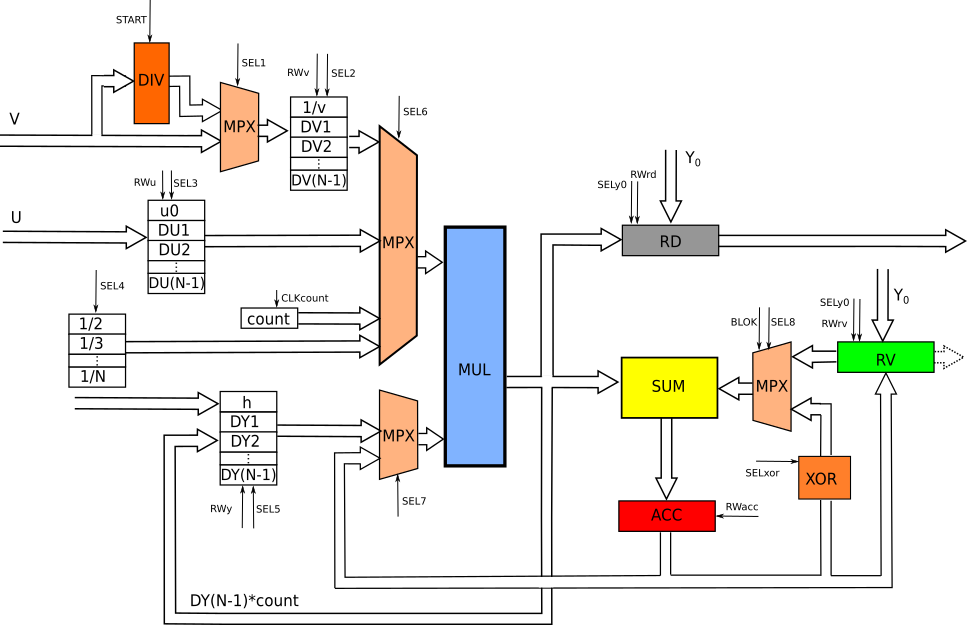
\includegraphics{obrazky/ppdi.png}}
\caption{Paralelno-paralelný deliaci integrátor \cite{MatecnyBP}.}
\label{ppdi}
\end{figure}
\bigskip



% Please add the following required packages to your document preamble:
% \usepackage[table,xcdraw]{xcolor}
% If you use beamer only pass "xcolor=table" option, i.e. \documentclass[xcolor=table]{beamer}
\begin{table}[H]
\centering
\begin{tabular}{|
>{\columncolor[HTML]{DAE8FC}}l |l|}
\hline
\multicolumn{1}{|c|}{\cellcolor[HTML]{68CBD0}{\color[HTML]{000000} \textbf{Skratka}}} & \multicolumn{1}{c|}{\cellcolor[HTML]{68CBD0}{\color[HTML]{000000} \textbf{Popis}}} \\ \hline
\textbf{V, U} & vstupné operandy integrátora \\ \hline
\textbf{1/v, DV1, ... DV(N-1)} & set registrov jednotlivých členov vstupného operandu V \\ \hline
\textbf{u0, DU1, ... DU(N-1)} & set registrov jednotlivých členov vstupného operandu U \\ \hline
\textbf{count} & čítač cyklov výpočtu - N \\ \hline
\textbf{1/2, 1/3, ... 1/N} & set registrov s jednotlivými podielmi \\ \hline
\textbf{h, DY1, ... DY(N-1)} & set registrov s krokom metódy a s vypočítanými členmi \\ \hline
\textbf{DIV} & delička \\ \hline
\textbf{XOR} & invertovanie hodnoty v dvojkovom doplnku (xor +1) \\ \hline
\textbf{MPX} & multiplexor 2-1, 4-1 \\ \hline
\textbf{START} & povoľovací signál na spustenie výpočtu \\ \hline
\textbf{SEL1, SEL6, SEL7, SEL8} & riadiace signály multiplexorov \\ \hline
\textbf{SEL2, SEL3, SEL4, SEL5} & riadiace signály registrov \\ \hline
\textbf{SELxor} & signál na invertovanie vstupnej hodnoty \\ \hline
\textbf{CLKcount} & signál na zvýšenie hodnoty čítača \\ \hline
\textbf{RWv, RWu, RWy} & povoľovacie signály sád registrov (READ/WRITE) \\ \hline
\end{tabular}
\caption{Význam skratiek v obrázku \ref{ppdi}.}
\label{my-label}
\end{table}




Podobne ako pri násobiacom integrátore, aj pri paralelnom deliacom integrátore sú na začiatku výpočtu vynulované registre pomocou signálu \textit{RESET} a nastavené signály multiplexorov \textit{MPX}. Ďalej je do registrov \textit{RD} a \textit{RV} nahraná počiatočná podmienka a do registra $ h $ je nahraný integračný krok. Do registrov $ 1/n $ sú uložené predvypočítané konštanty. Po prijatí hodnôt $ U $ a $ V $ sa začne výpočet. Hodnota $ V $ je privedená do deličky $ DIV $ a spustí sa výpočet $ 1/v $ s~použitím deliaceho algoritmu \textit{SRT}. Delenie je realizované len raz počas celého výpočtu, keďže ide o~veľmi náročnú operáciu. Po skončení operácie delenia je výsledok uložený do setu registrov $ DVN $, a to konkrétne do registra $ 1/v $. V ďalšom cykle výpočtu je vstupná hodnota $ V $ privedená priamo do setu registrov $ DVN $ bez delenia. Hodnota $ U $ je uložená do setu registrov $ DUN $. Pre optimalizáciu je paralelne s~delením realizovaný výpočet násobenia $ uh $. Po skončení výpočtu je výsledok aktuálneho člena uložený do registra \textit{RD} a privedený na výstup deliaceho integrátora. Suma jednotlivých členov je postupne ukladaná v každom cykle do registra $ RV $, z ktorého je možné získať hodnotu privedenú na výstup, rovnako ako aj v násobiacom integrátore.


\section{Návrh jednovstupového integrátora}
Tento integrátor bol navrhnutý podľa rovníc \eqref{DY_cleny}, na základe ktorých počíta diferenciálnu rovnicu \eqref{jednoducha_rovnica}. Z toho vyplýva, že vykonáva numerickú integráciu vstupnej hodnoty, a následne výslednú hodnotu posiela na výstup. Schéma integrátora je na obrázku \ref{ppi_fp} a vychádza z práce J. Opálku \cite{OpalkaBP}. Na naštartovanie výpočtu slúži počiatočná podmienka. Tá je nahraná na začiatku výpočtu do registra \textit{RV}. Následne je cez multiplexor \textit{MPX} privedená a uložená do registra \textit{RD}. V sete registrov $ h $ je uložený integračný krok metódy a jeho podiely. Rovnako ako v predchádzajúcich prípadoch je možné počet registrov znížiť na polovicu. Vstupnú hodnotu $ Z $ nie je potrebné ukladať do registrov, keďže sa nepoužíva pri výpočte ďalších členov. Jednotlivé hodnoty členov sú ukladané do registra \textit{RV} a poslané na výstup integrátora. Ak chceme získať výslednú hodnotu Taylorovej rady rovnice \eqref{jednoducha_rovnica}, stačí priviesť hodnotu z registra \textit{RV} cez multiplexor \textit{MPX} do registra \textit{RD}, kde je hodnota sprístupnená na výstupe integrátora.


\bigskip
\begin{figure}[h]
\centering
\scalebox{0.4}{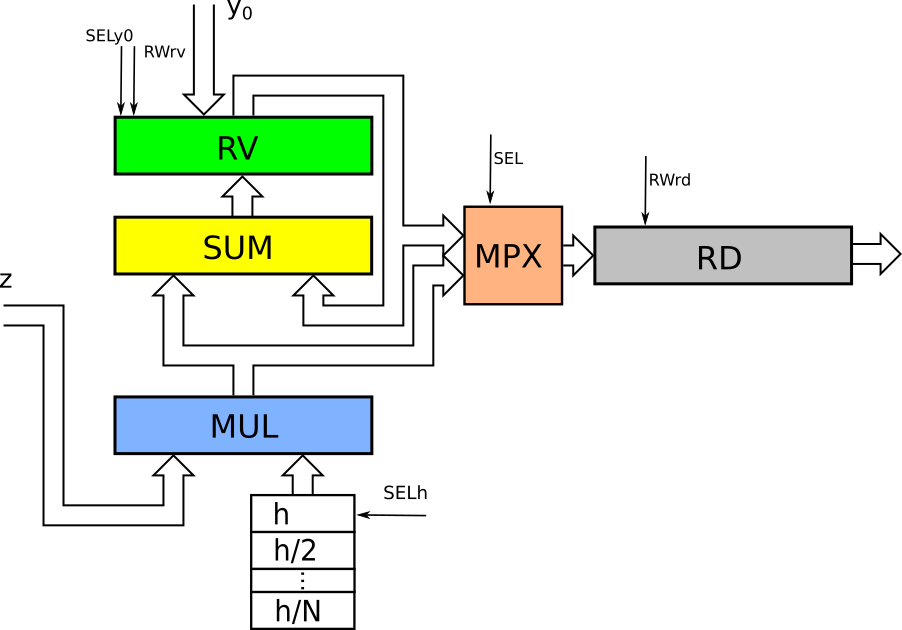
\includegraphics{obrazky/ppi.png}}
\caption{Paralelný jednovstupový integrátor v pohyblivej rádovej čiarke.}
\label{ppi_fp}
\end{figure}
\bigskip

\section{Návrh komponentu na spracovanie exponentov}
V pohyblivej rádovej čiarke sú operácie násobenia, delenia a sčítania (odčítania) zložitejšie, nakoľko je k týmto operáciám pridaná aj práca s výpočtom znamienka, exponentu a mantisy. Výpočet exponentov je možné vykonávať v každom z komponentov (násobička, delička, sčítačka) samostatne, alebo pomocou jedného komponentu spoločného pre tieto komponentmi. Pri spoločnom komponente je možné znížiť priestorovú zložitosť zapojenia. Tým sa však zvýši  náročnosť synchronizácie a riadenia kontrolóra. V deliacom integrátore to môže spôsobiť zdržanie výpočtu vtedy, keď sa operácia delenia a násobenia vykonávajú paralelne. Avšak táto situácie nastane len raz, na začiatku výpočtu. Predošlé popísané návrhy násobiaceho, deliaceho a jednovstupového integrátora je možné použiť ako pri implementácii v pevnej rádovej čiarke, tak aj v pohyblivej rádovej čiarke. Integrátory v pohyblivej rádovej čiarke vychádzajúce z popísaných návrhov pracujú s exponentami v každej operácii samostatne.
V nasledujúcich sekciách si popíšeme druhý variant spracovania exponentu so spoločným komponentom.

Blokové schémy zapojenia integrátorov pracujúcich v~pohyblivej rádovej čiarke vychádzajú z~predchádzajúcich návrhov. Boli však rozšírené o~prácu so znamienkami, s~mantisou a s~exponentmi. Samotný výpočet exponenta sa deje v spoločnom komponente \textit{EXP}, ktorého návrh je zobrazený na obrázku~\ref{ppi_fp_exp}.

\bigskip
\begin{figure}[h]
\centering
\scalebox{0.8}{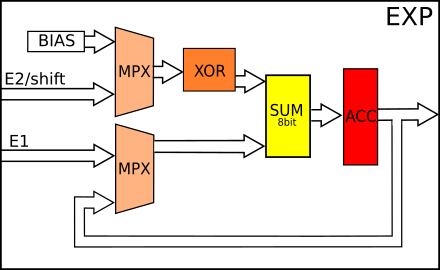
\includegraphics{obrazky/ppdi_fp_exp.png}}
\caption{EXP - blok pracujúci s~exponentmi.}
\label{ppi_fp_exp}
\end{figure}
\bigskip


% Please add the following required packages to your document preamble:
% \usepackage[table,xcdraw]{xcolor}
% If you use beamer only pass "xcolor=table" option, i.e. \documentclass[xcolor=table]{beamer}
\begin{table}[H]
\centering
\begin{tabular}{|
>{\columncolor[HTML]{DAE8FC}}l |l|}
\hline
\multicolumn{1}{|c|}{\cellcolor[HTML]{68CBD0}{\color[HTML]{000000} \textbf{Skratka}}} & \multicolumn{1}{c|}{\cellcolor[HTML]{68CBD0}{\color[HTML]{000000} \textbf{Popis}}} \\ \hline
\textbf{E1} & vstupná hodnota väčšieho exponenta \\ \hline
\textbf{E2/shift} & vstupná hodnota menšieho exponenta/hodnota posunu \\ \hline
\textbf{BIAS} & hodnota 127 alebo 2047 \\ \hline
\textbf{SUM (8/11bit)} & paralelná 8 alebo 11 bitová sčítačka \\ \hline
\textbf{INV} & invertor \\ \hline
\end{tabular}
\caption{Význam skratiek použitých v obrázku \ref{ppi_fp_exp}.}
\label{my-label}
\end{table}

Komponent \textit{EXP} slúži na vykonávanie výpočtov s~exponentmi, ktoré sú popísané v~sekciách~\ref{PlusMinusFP} a~\ref{MulDivFP}. Obsahuje dva vstupy, do ktorých sú privedené jednotlivé exponenty z~komponentov $ DIV $, $ MUL $ a $ SUM $ a jeden výstup. Celý komponent \textit{EXP} pracuje na počte bitov, ktorý sa rovná veľkosti exponenta, ktorá je závislá od použitej aritmetiky. Pri jednoduchej presnosti (32 bitov) je veľkosť exponenta 8 bitov a pri dvojitej presnosti (64 bitov) na 11 bitov. Komponent teda obsahuje buď 8-bitovú alebo 11-bitovú sčítačku a ostatné komponenty v rovnakej bitovej šírke.
Pri vykonávaní operácie súčinu alebo rozdielu slúži komponent \textit{EXP} na výpočet rozdielu exponentov. Výsledná hodnota rozdielu je privedená naspäť do sčítačky \textit{SUM} cez register \textit{ACC}. O túto hodnotu je následne v sčítačke posunutá hodnota mantisy menšieho čísla doprava. Výsledná hodnota mantisy je potom súčet/rozdiel mantisy väčšieho čísla a posunutej mantisy. Znamienko a exponent sa rovnajú hodnote väčšieho čísla z počítaných operandov.
Pri operácii delenia alebo násobenia slúži komponent \textit{EXP} na výpočet výsledného exponenta. Podľa typu operácie sa vykoná súčet alebo rozdiel prijatých exponentov. Táto hodnota je uložená v~registri \textit{ACC} a privedená naspäť do sčítačky $ SUM_{8/11bit} $ s~hodnotou z~registra $ BIAS $. Vykoná sa súčet alebo rozdiel týchto hodnôt. Získame tak hodnotu nového exponenta, ktorá je privedená naspäť do násobičky $ MUL $ alebo deličky $ DIV $. Ak je však po delení alebo násobení potrebné vykonať posun mantisy, hodnota vypočítaného exponentu je privedená z \textit{ACC} cez multiplexor \textit{MPX} naspäť do sčítačky  $ SUM_{8/11bit} $, a na vstup \textit{E2/Shift} je privedená hodnota posunu. Vykoná sa rozdiel hodnôt, čím vykonáme posun exponenta. Následne je výsledná hodnota privedená do násobičky $ MUL $ alebo deličky $ DIV $ a použitá ako nová hodnota exponentu.

Kvôli prehľadnosti schéma neobsahuje znázornenie zapojenia výpočtu znamienka a rozdelenie operandov na znamienko, exponent a na mantisu, a ich opätovné zloženie. Tieto operácie sa vykonávajú v~komponentoch \textit{DIV}, \textit{MUL} a \textit{SUM}.\\

\section{Návrh násobiacieho integrátora v~pohyblivej rádovej čiarke}
Návrh paralelného násobiaceho integrátora v~pohyblivej rádovej čiarke so spoločným komponentom \textit{EXP} je na obrázku~\ref{ppni}. Čísla v~pohyblivej rádovej čiarke môžeme zobraziť presnejšie ako čísla v~pevnej rádovej čiarke, čiže pri uložení malých čísel v~pohyblivej rádovej čiarke dochádza k~menšej zaokrúhľovacej chybe. Z~tohoto dôvodu je možné počítať Taylorovu radu s~použitím väčšieho počtu členov a zvýšiť tak presnosť výpočtu. Integrátory v~pohyblivej rádovej čiarke teda môžu počítať viac členov Taylorovej rady, a teda počet registrov $ DR(N-1) $ a $ DQ(N-1) $ sa zvýši. Set registrov $ h/i, i=2,3..N $ obsahuje \textit{N-1} registrov. Počet týchto registrov je možné znížiť rovnako ako pri integrátoroch v~pevnej rádovej čiarke.

\begin{figure}[h]
\centering
\scalebox{0.6}{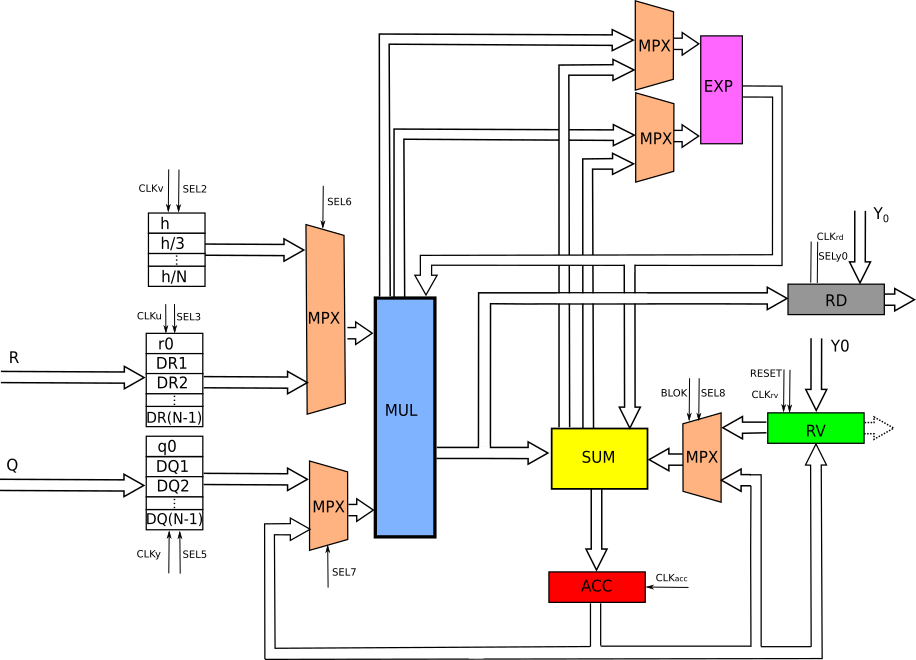
\includegraphics{obrazky/ppni_fp40.png}}
\caption{Paralelno-paralelný násobiaci integrátor v~pohyblivej rádovej čiarke}
\label{ppni_fp}
\end{figure}
\bigskip

Spôsob výpočtu paralelného násobiaceho integrátora v~pohyblivej rádovej čiarke so spoločným komponentom \textit{EXP} je takmer rovnaký ako pri násobiacom integrátore v~pevnej rádovej čiarke. Rozdielne sa vykonávajú operácie násobenia a sčítania. Po privedení hodnôt na vstupy násobičky $ MUL $ alebo sčítačky $ SUM $ sú čísla v~FP uložené do pomocných registrov v~týchto komponentoch. Z~týchto registrov sú jednotlivé časti FP čísla rozdistribuované do samostatných výpočtových obvodov. V komponente \textit{MUL} sú znamienka privedené ku komponentu $ XOR $, ktorý vykonáva nonekvivalenciu. V komponente \textit{SUM} sa výsledné znamienko rovná znamienku väčšieho čísla zo vstupných hodnôt. Exponenty, ako je popísané vyššie, spracúva komponent $ EXP $. Mantisy sú privedené do paralelnej násobičky alebo sčítačky. Veľkosť výsledku násobičky je dvojnásobná veľkosti mantisy so skrytou jednotkou, t. j. 48 bitov pri jednoduchej presnosti a 106 bitov pri dvojitej presnosti. Veľkosť sčítačky sa rovná veľkosti mantisy so skrytou jednotkou, t. j. 24 alebo 53 bitov. Výsledné hodnoty jednotlivých častí čísla v pohyblivej rádovej čiarke sú na výstupe spojené do jedného čísla a sú uložené do výstupného registra daného komponentu ($ MUL $ alebo $ SUM $). Následne sú poskytnuté na jeho výstupe k~ďalšiemu výpočtu.

\section{Deliaci integrátor v~pohyblivej rádovej čiarke}
Paralelný deliaci integrátor v~pohyblivej rádovej čiarke so spoločným komponentom \textit{EXP} je najzložitejší z~navrhnutých integrátorov. Obsahuje všetky spomínané operácie: sčítanie, odčítanie, násobenie a delenie; a všetky vykonáva v~pohyblivej rádovej čiarke, v ktorej je práca s exponentami vykonávaná v jednom komponente \textit{EXP}.
Operácie násobenia a sčítania sa vykonávajú rovnako ako v~paralelnom násobiacom integrátore v~pohyblivej rádovej čiarke. Operácia delenia sa vykonáva iba raz za celý výpočet, a to paralelne s~operáciou násobenia, ako aj v~deliacom integrátore s~FX aritmetikou. Tu však môže dôjsť ku kolízii v~použití komponentu $ EXP $, keďže delenie je náročnou operáciou, pričom dĺžka výpočtu záleží na použití daného algoritmu. Podľa zvoleného algoritmu je potom potrebné zvoliť, ktorá operácia bude mať prednosť v použití komponentu $ EXP $. Po uvoľnení $ EXP $ násobičkou $ MUL $ je komponent $ EXP $ pridelený deličke $ DIV $ na výpočet exponentov. Ak je použitý zdĺhavejší algoritmus pri výpočte delenia (napr. SRT algoritmus použitý v deliacom integrátore vo FX aritmetike), čiže ak operácia delenia trvá dlhší čas ako operácia násobenia, je vhodnejšie prenechať komponentu \textit{EXP} najprv operácii násobenia. Ak je deliaci algoritmus veľmi rýchly a čas výpočtu je podobný času výpočtu operácie násobenia, tak potom nezáleží, ktorý z komponentov bude ako prvý využívať \textit{EXP}. Po skončení delenia je podiel uložený do registra $ 1/v $ a pokračuje sa v~ďalšom výpočte.
Výpočet prebieha podobne ako pri deliacom integrátore bez komponentu \textit{EXP}. Rozdielne sa vykonávajú operácie delenia, násobenia a sčítania. Ďalší rozdiel je v komponente \textit{XOR}, ktorý bol nahradený komponentom \textit{INV}. Prevrátenie hodnoty čísla sa v pevnej rádovej čiarke použitím doplnkového kódu deje operáciou $ XOR $ a pričítaním jednotky, ako to je v predchádzajúcom deliacom integrátore. V pohyblivej rádovej čiarke sa však invertovanie hodnoty čísla vykonáva jednoduchým invertovaním znamienkového bitu $ S $ vstupného operandu. Toto invertovanie sa vykonáva v spomínanom komponente \textit{INV}.

\begin{figure}[h]
\centering
\scalebox{0.55}{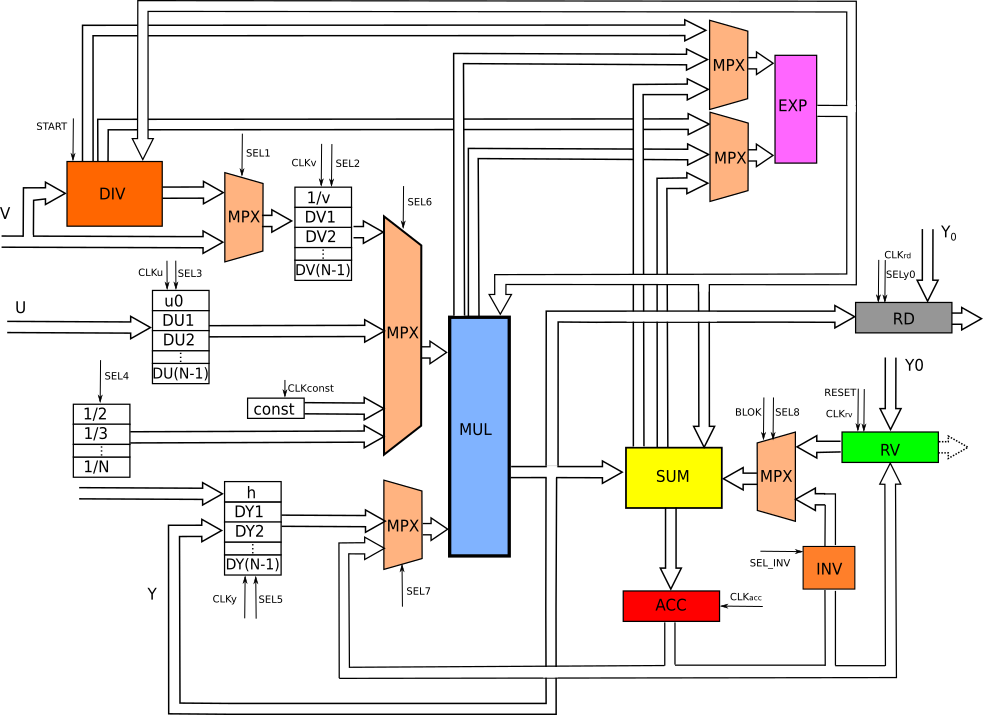
\includegraphics{obrazky/ppdi_fp.png}}
\caption{Paralelno-paralelný deliaci integrátor v~pohyblivej rádovej čiarke}
\label{ppdi_fp}
\end{figure}
\bigskip

\newpage
\section{Sústava diferenciálnych rovníc} \label{navrhSustava}
Integrátory, ktoré sme si popísali, je možné medzi sebou zapojiť, a riešiť tak diferenciálnu rovnicu. Po zapojení integrátorov nebude nutné predvypočítať vstupné hodnoty, stačí len zadať počiatočné podmienky na naštartovanie výpočtu a všetky ostatné hodnoty sa dopočítajú.
Zvoľme konkrétnu diferenciálnu rovnicu s operáciou násobenia v tvare
\begin{eqnarray}
y' & = & \sin(t) e^{-t} \, , \quad y(0) = 1 . \label{dif_sint_et}
\end{eqnarray}
\bigskip

Rovnicu prevedieme do sústavy diferenciálnych rovníc:
\begin{eqnarray}
y' & = & qr \, , \quad y(0) = 1 \nonumber \\
r' & = & -r \, , \quad r(0) = 1 \\
q' & = & s \, , \quad q(0) = 0 \nonumber \\
s' & = & -q \, , \quad s(0) = 1 . \nonumber
\end{eqnarray}

Zo sústavy rovníc vytvoríme schému zapojenia integrátorov, znázornenú na obrázku \ref{ppi_fp_sustava}. Schému tvoria tri jednovstupové integrátory \textit{r}, \textit{q} a \textit{s}, dvojvstupový násobiaci integrátor \textit{y} a dva invertory. Invertor je komponent, ktorý invertuje prichádzajúcu hodnotu. Integrátor \textit{r} a invertor tvoria spolu funkciu $ e^{-t} $. Integrátory \textit{r}, \textit{s} a invertor tvoria spolu funkciu $ sin(t) $. Nakoniec sú tieto hodnoty privádzané na vstup násobiaceho integrátora \textit{y}, ktorý počíta diferenciálnu rovnicu \ref{dif_sint_et}.
TODO rovnicu s deliacim integrátorom.
Zo schémy zapojenia je možné následne vytvoriť VHDL kód a vykonať výpočet na FPGA. Takýto postup je vhodný pre rozsiahle diferenciálne rovnice s väčším počtom operácií, ktorých výpočet by bol vykonávaný veľmi často. Ako vhodnejší spôsob použitia sa ponúka prepojovacia sieť medzi rôznymi integrátormi. Pred výpočtom by sa sieť nakonfigurovala podľa danej diferenciálnej rovnice a výpočet by mohol prebiehať bez nutnosti syntézy. Tento variant je síce priestorovo náročný, ale ponúka variabilitu výpočtu.
V ďalšej kapitole si predstavíme implementáciu popísaných integrátorov a taktiež implementáciu sústavy diferenciálnych rovníc pomocou metódy bez použitia prepojovacej siete.
\bigskip

\begin{figure}[h]
\centering
\scalebox{0.5}{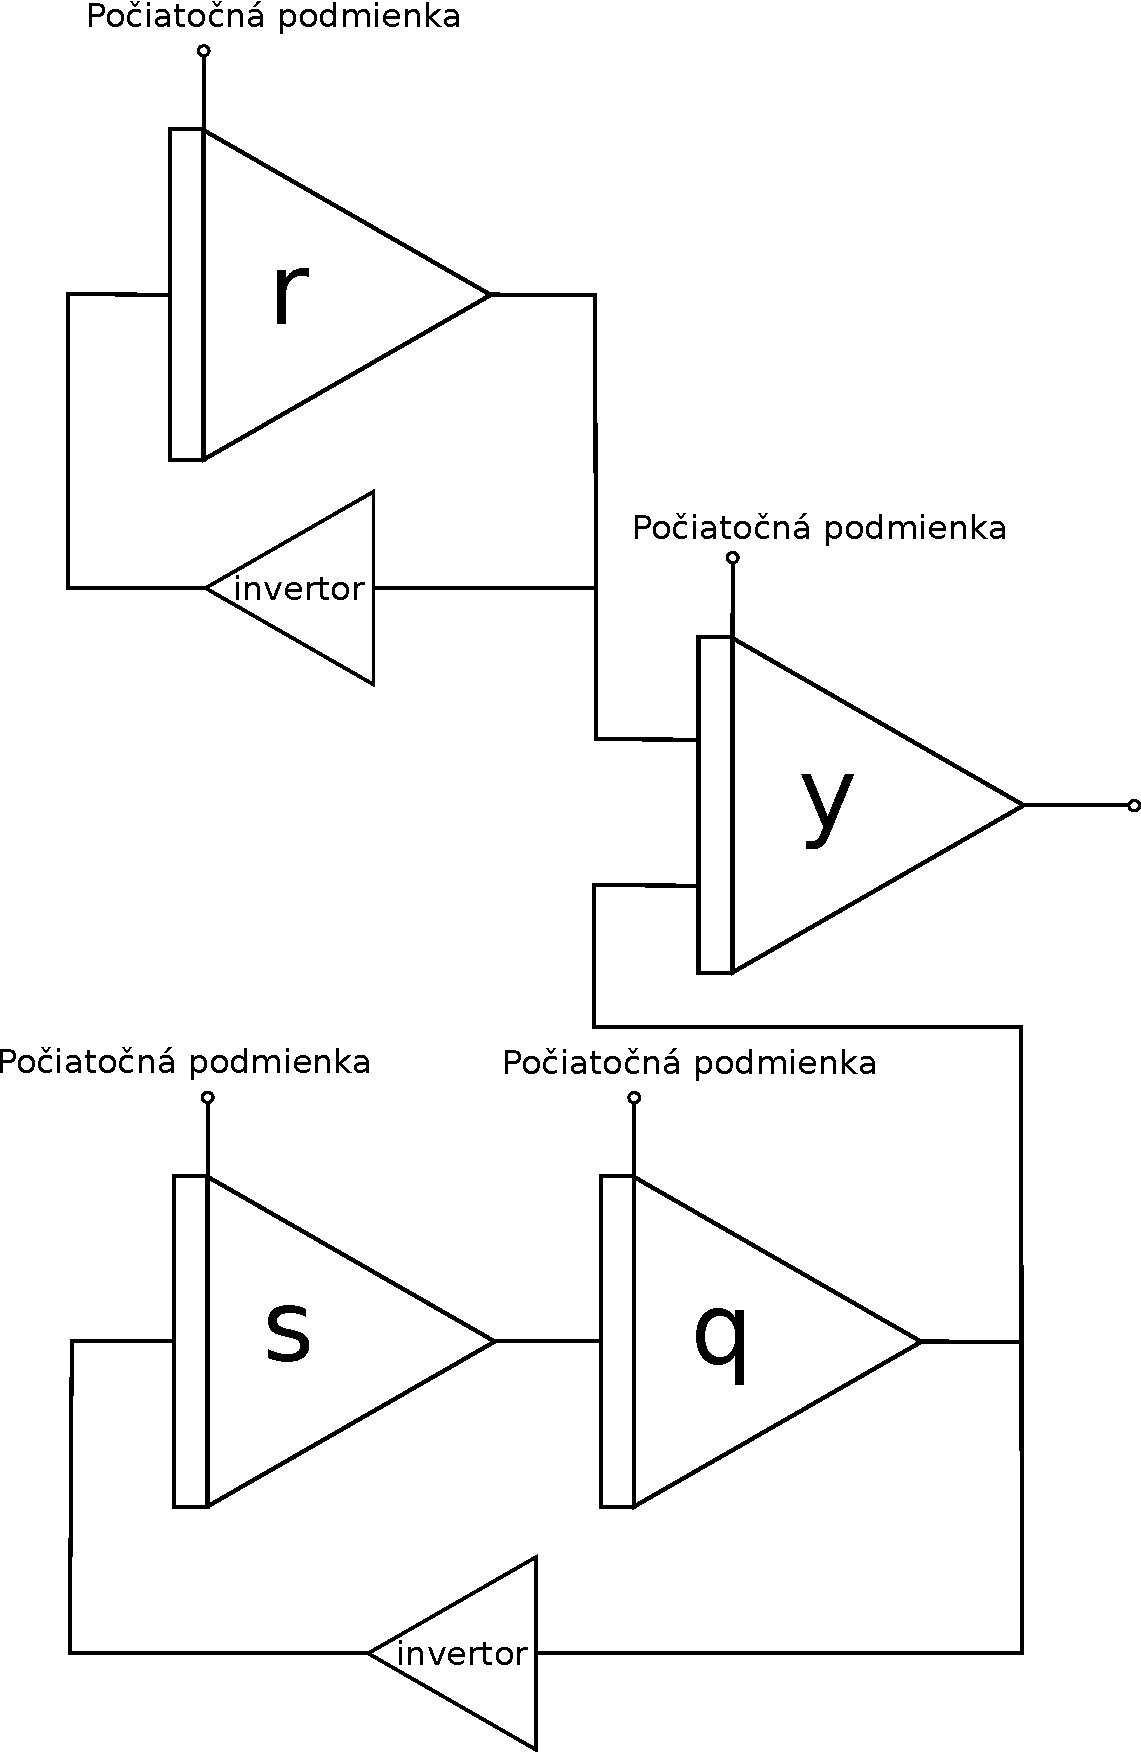
\includegraphics{obrazky/sustava_integratorov.pdf}}
\caption{Schéma zapojenia integrátorov \cite{MatecnyBP}}
\label{ppi_fp_sustava}
\end{figure}
\bigskip



\chapter{Popísanie integrátorov vo VHDL} \label{IMPLEMENTACIA}
Jednotlivé integrátory predstavené v kapitole \ref{NUM_INTEGRATORY} boli popísané v jazyku VHDL v prostredí Xilinx ISE a následne odsimulované v nástroji Model Sim s pomocou použitia \textit{testbanchu}. Potom boli niektoré z integrátorov otestované na programovateľnom hradlovom poli FPGA.
Pre priestorovú zložitosť paralelných integrátorov bola snaha implementovať integrátory na rozsiahlejšom čipe FPGA, a to konkrétne na VIRTEX-5 s čipom XC5VSX50T. Pre prácu s týmto čipom je potrebná plná verzia programu Xilinx ISE s licenciou. Poskytnutie licencie od VUT FIT pre študenta však nie je možné. Riešením nakoniec bolo použitie licencie pomocou pripojenia sa na fakultnú sieť cez VPN. Následne bol integrátor implementovaný na VIRTEX-5, avšak skončenie výpočtu bolo možné zistiť len rozsvietením diódy, čo je nepoužiteľný spôsob na získanie hodnoty výsledku. Preto bolo snahou výsledok zobraziť na LCD displeji, prípadne vytvoriť komunikáciu cez terminál. Sprevádzkovanie displeja podľa rôznych návodov bolo neúspešné a pre komunikáciu s terminálom bolo potrebné doinštalovať ďalšie programy. Vzhľadom na dané komplikácie bolo teda nutné použiť iný čip, a to konkrétne FPGA Spartan 3 XC3S50, ktorý je použitý v študijnej pomôcke FitKit 2.0. Veľkosť tohto FPGA je však veľmi malá, a ani jeden z navrhnutých integrátorov nie je možné naprogramovať na tento čip. Po konzultácii s Ing. Václavom Šimekom sme začali pracovať s prípravkom FitKit 2.0 s vymeneným FPGA za väčší, a to za Spartan 3 XC3S400. Práca s týmto FPGA je kompatibilná s predchádzajúcim čipom, a preto bolo možné na programovanie použiť nástroj QDevKit. Ide o multiplatformový terminálový program pre jednoduchú prácu s FitKitom. Všetky parametre sú už v programe nastavené a komunikácia prebieha cez USB namiesto emulovaného sériového portu, ako je to pri iných terminálových programoch. Informácie o FitKite, o programe QDevKit a taktiež návody na vytvorenie vlastnej aplikácie boli čerpané z webstránky FitKitu \cite{fitkit}.
Na FitKite bol odskúšaný jednovstupový integrátor s 32 bitovou fixed point a floating point aritmetikou. Tento integrátor bol vybraný pre jeho najmenšiu priestorovú zložitosť. Ďalej bol implementovaný integrátor počítajúci rovnicu \ref{rovnica}. Integrátor pracuje na 32 bitoch a používa FX aritmetiku. Rovnica je počítaná Taylorovou radou 4. rádu. Ostatné integrátory a verzie integrátorov nie je možné nahrať na FPGA, ktoré je použité vo FitKite.

Jednotlivé časti integrátorov boli popísané samostatne a následne bola vytvorená štruktúra vzájomného prepojenia, ktorá tvorí celý integrátor. Pri každom integrátore sú jednotlivé kroky výpočtu riadené kontrolórom. Ten je tvorení cyklickým konečným automatom. Cyklus vyplýva z rovníc \eqref{suma_mul} a \eqref{suma_div}, keďže výpočet jednotlivých členov je podobný, avšak so zväčšujúcim sa počtom operácií. Samozrejme, po skončení výpočtu je možné pomocou signálu $ RESET $ prejsť do počiatočného stavu a zadaním novej počiatočnej podmienky začať nový výpočet. Ďalej podrobnejšie popíšeme jednotlivé integrátory.

\section{Integrátory v pevnej rádovej čiarke}
Všetky integrátory v pevnej rádovej čiarke (t. j. deliaci, násobiaci a jednovstupový integrátor) kódujú čísla v dvojkovom kóde. Použité sčítačky a násobičky sú paralelné a výpočet operácie trvá jeden hodinový takt. Pri výpočte je však potrebné použiť dva takty, aby došlo k ustáleniu signálov: jeden na nastavenie signálov a druhý na uloženie výsledku.

\subsubsection*{Násobiaci integrátor}

Paralelný dvojvstupový násobiaci integrátor vo fixpoint aritmetike bol implementovaný v dvoch verziách, a to na 32 a 64 bitoch. Veľkosť použitej aritmetiky je však možné jednoducho zväčšiť, keďže celý kód je písaný genericky. Taktiež je možné zmeniť počet cyklov výpočtu, čiže počet počítaných členov Taylorovej rady, avšak v závislosti od počtu cyklov $ N $ je nutné upraviť počet registrov v registrových setoch. Pri násobiacom integrátore sú to sety registrov \textit{DQ(N-1)}, \textit{DR(N-1)} a počet registrov $ h/i $, kde $ i = 2..N $. Pri deliacom integrátore je potrebné zväčšiť počet registrov \textit{DV(N-1)}, \textit{DU(N-1)} a \textit{1/i}, kde $ i = 2..N $. S tým súvisí potreba následného zväčšenia bitovej šírky riadiacich signálov označovaných s prefixom \textit{SEL}. Bitovú šírku signálov je vhodné zvoliť z počtu $ N $ registrov podľa vzťahu \textit{šírka registrov} $ = \log_{2} N $ a využiť tak celú šírku a kombinácie binárneho kódovania.

Pre 32 i 64 bitovú verziu bola použitá FX aritmetika, ktorá je názorne zobrazená na obrázku \ref{fxmularitmetic}. Aritmetika je tvorená s jedným znamienkovým bitom, s 1 bitom pred desatinnou čiarkou a s $ m $ bitmi za desatinnou čiarkou. Pri jednoduchej presnosti sa $ m $ rovná 30 bitom a pri dvojitej presnosti sa $ m $ rovná 62 bitom. Výpočet počíta s Taylorovou metódou 8. rádu, a teda výpočet prebieha až po 8. člen Taylorovej rady, t. j. DY8.

\bigskip
\begin{figure}[h]
\centering
\scalebox{0.3}{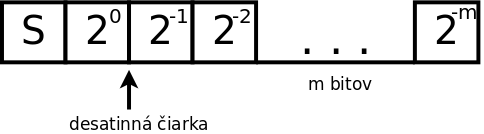
\includegraphics{obrazky/FXmularitmetika.png}}
\caption{FX aritmetika numerického integrátora.}
\label{fxmularitmetic}
\end{figure}
\bigskip

Násobiaci integrátor je ovládaný pomocou kontrolóra. Jednotlivé stavy kontrolóra a nastavenia signálov sú uvedené v tabuľke \ref{kontrolermulfx}. Kontrolór obsahuje 9 stavov a dva čítače \textit{count} a \textit{countQ}. Čítač \textit{count} udáva číslo aktuálneho cyklu a \textit{countQ} je v každom cykle nastavený na hodnotu \textit{count} a postupne sa dekrementuje. Výpočet začína nastavením signálu \textit{reset} na logickú 1. To spôsobí prepnutie násobiaceho integrátora do stavu s rovnakým názvom, čiže \textit{Reset}. V ňom sa integrátor uvedie do počiatočného stavu. Vynulujú sa počítadlá a čaká sa na povoľovací signál \textit{EN}, ktorým sa prepne integrátor do stavu \textit{Init}. V tomto stave je nahraná počiatočná podmienka a sú uložené vstupné hodnoty. Výpočet prejde do stavu \textit{MulDQxDRx}. V ňom sú vynásobené jednotlivé členy \textit{DQi} a \textit{DRj}, kde $ i, j $ značí aktuálne počítaný člen. Z rovnice \eqref{suma_mul} vyplýva, že sa vykonáva násobenie kombinácií týchto členov. Na to slúžia spomenuté čítače \textit{count} a \textit{countQ}. Na základe čítačov sa nastavia signály \textit{SELR} a \textit{SELQ}. Po vynásobení členov je výsledok v stave \textit{WriteAcc} uložený do akumulátora. Zo stavu \textit{WriteAcc} je integrátor prepnutý buď do stavu \textit{SetupCounter}, alebo do stavu \textit{MulAccH\_RV}. V stave \textit{SetupCounter} sa dekrementuje počítadlo \textit{countQ} a začína sa násobenie ďalšej kombinácie členov \textit{DQi} a \textit{DQj}. Ak sú vynásobené všetky kombinácie týchto členov, stačí potom už len vynásobiť obsah akumulátora hodnotou $ h/N $. Integrátor je teda prepnutý do stavu \textit{MulAccH\_RV} a vykoná sa operácia násobenia. Výsledok je uložený do registra \textit{RD} (nejde o variantu \uv{posledného} integrátora v zapojení). Potom je v stave \textit{SaveToAcc} sčítaná hodnota s hodnotou registra \textit{RV} a následne je uložená do akumulátora. V ďalšom stave \textit{SaveToRv} je výsledok v \textit{ACC} uložený do registra \textit{RV}. Výpočet končí v stave \textit{Result}, v ktorom je nastavený signál \textit{OEN} (output enable) na logickú jednotku. Po nastavení povoľovacieho signálu \textit{EN} na logickú jednotku je výpočet znova spustený s novými hodnotami.

\subsubsection*{Deliaci integrátor}

Paralelný deliaci integrátor vo fixpoint aritmetike bol implementovaný, podobne ako násobiaci integrátor, v 32 a 64 bitovej verzii. Pri návrhu integrátorov sa kládol dôraz nielen na rýchlosť výpočtu, ale aj na priestorovú zložitosť. 
Z rovnice \eqref{suma_div} vyplýva, že členy $ DYN $ sú násobené číslom $ N-k $, kde $ k $ je minimálne 1, a teda najväčšie číslo je $ N-1 $. Aby bolo možné toto číslo zobraziť, bolo potrené zvoliť vhodnú aritmetiku, t. j. vhodný počet čísel pred a za desatinnou čiarkou. Čím väčší počet bitov sa nachádza pred desatinou čiarku, tým viac sa zväčšuje interval zobraziteľných čísel, avšak zmenšuje sa počet bitov za desatinnou čiarkou. Pri zmenšovaní počtu čísel za desatinnou čiarkou sa zmenšuje hustota zobrazenia čísel a v konečnom dôsledku aj ich presnosť. V dvojkovom doplnkovom kóde pri 1 bite pred desatinou čiarkou sme schopný vypočítať deliacim integrátorom maximálne dva členy Taylorovej rady. Pri dvoch bitoch sú to 4 členy, pri troch bitoch 8 členov Taylorovej rady a pri štyroch bitoch 16 členov Taylorovej rady. To je možné vyjadriť ako $ N = 2^{w} $, kde \textit{N - počet členov, w - bitová šírka}. Keďže pri použití Taylorovej metódy 4. rádu nemusí byť riešenie dostatočné presné, 32 bitová verzia integrátora počíta s Taylorovou metódou 8. rádu, a teda je použitá aritmetika s jedným znamienkovým bitom, s tromi bitmi pred desatinnou čiarkou. Ostatných 28 bitov tvorí časť za desatinnou čiarkou. Vyšší rád metódy nie je použiteľný, keďže hodnoty vyšších členov by boli veľmi malé, a teda nezobraziteľné v danej aritmetike. Táto aritmetika je zobrazená na obrázku \ref{fxdivaritmetic32}.

\bigskip
\begin{figure}[h]
\centering
\scalebox{0.3}{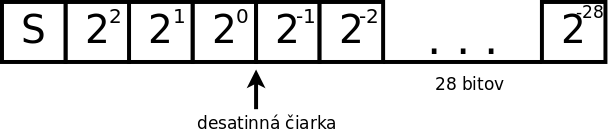
\includegraphics{obrazky/FXdivaritmetika32.png}}
\caption{FX aritemtika deliaceho integrátora na 32 bitoch.}
\label{fxdivaritmetic32}
\end{figure}
\bigskip


\bigskip
\begin{figure}[h]
\centering
\scalebox{0.3}{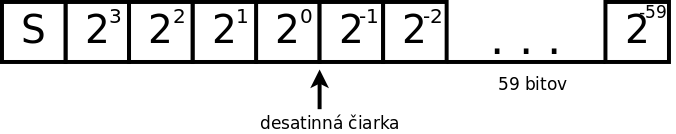
\includegraphics{obrazky/FXdivaritmetika64.png}}
\caption{FX aritmetika deliaceho integrátora na 64 bitoch.}
\label{fxdivaritmetic64}
\end{figure}
\bigskip

V 64 bitovej verzií deliaceho integrátora ponúka väčšiu bitovú šírku a teda aj presnosť, preto bola veľkosť použitých bitov pred desatinnou čiarkou zväčšená o jeden bit. Za desatinnou čiarkou sa potom nachádza 59 bitov. V tejto verzií deliaceho integrátora sme teda schopný vypočítať v danej aritmetike až 16 členov Taylorovej rady. Použité aritmetika je na obrázku \ref{fxdivaritmetic64}.

Postup výpočtu delaiceho integrátora je podobný ako v násobiacom integrátore. Jendotlivé stavy kontroléra a nastavenie signálov sú uvedené v tabuľke \ref{kontrolerdivfx}. Začiatok výpočtu je rovnaký ako u integrátora s operáciou násobenia. Integrátor je v počiatočnom stave t.j. v stave \textit{Reset}. Z neho prejde do stavu \textit{Init}. Následne v stave \textit{MulUH} je násobená hodnota člena \textit{DUi} a s integračným krokom \textit{h}. Výsledok je uložený do akumulátora \textit{ACC}. Výsledok násobenia je možné uložiť už v tomto kroku, kedže nastavenie signálov multiplexorov a výpočet násobenia bolo možné začať už v stave \textit{Init}. Paralelne s operáciou násobenia je signálom \textit{START} zahájené delenie \textit{1/v}, kde \textit{v} je vstupná hodnota operandu. Operácia delenia sa vykonáva pomocou SRT algoritmu s radixom 2. Bližšie informácie o danom algoritme a implmementácií môžeme nájsť v \cite{MatecnyBP}. V stave \textit{WaitDiv} je integrátor niekoľko cyklov, až kým sa neskončí operácia delenia. Delička po vykonaní operácie delenia nastavý výstupný signál \textit{done} na 1, čím umožní prechod integrátora do nasledujúceho stavu \textit{SaveDiv}. V ňom je hodnota delenia uložená do registra \textit{1/v}. Tým dostaneme hodnotu prvého člena Tylorovej rady. Hodnota je sčítaná s hodnotou registra \textit{RV} a uložaná naspäť do registra.


\begin{landscape}
\begin{table}[]
\scriptsize
\centering
\begin{tabular}{|l|c|c|c|c|c|c|c|c|c|c|l|}
\hline
\rowcolor[HTML]{68CBD0} 
\textbf{Stav}                                 & \textbf{SELy0} & \textbf{SEL1} & \textbf{SEL2} & \textbf{SEL3} & \textbf{SELQ} & \textbf{SELR} & \textbf{SELH} & \textbf{RWacc} & \textbf{RWrv} & \textbf{BLOK}           & \textbf{}                                                                             \\ \hline
\cellcolor[HTML]{DAE8FC}\textbf{Reset}        & 0              & 0             & 0             & 0             & 0             & 0             & 0             & 0              & 0             & 0                       & \begin{tabular}[c]{@{}l@{}}count = 0;\\ countQ = 0;\end{tabular}                      \\ \hline
\cellcolor[HTML]{DAE8FC}\textbf{Init}         & 1              & X             & X             & X             & X             & X             & X             & 0              & 1             & X                       & \begin{tabular}[c]{@{}l@{}}count = 0;\\ countQ = 0;\end{tabular}                      \\ \hline
\cellcolor[HTML]{DAE8FC}\textbf{MulDQxDRx}    & X              & 1             & 0             & 0             & countQ        & count-countQ  & X             & 0              & 0             & If countQ=count ? 1 : 0 & \begin{tabular}[c]{@{}l@{}}If count \textless N ? \\ WriteToAcc : Result\end{tabular} \\ \hline
\cellcolor[HTML]{DAE8FC}\textbf{WriteToAcc}   & X              & 1             & 0             & 0             & countQ        & count-countQ  & X             & 1              & 0             & If countQ=count ? 1 : 0 & \begin{tabular}[c]{@{}l@{}}If countQ = 0 ?\\ MulAccH\_RV : SetupCounter\end{tabular}  \\ \hline
\cellcolor[HTML]{DAE8FC}\textbf{SetupCounter} & X              & X             & X             & X             & X             & X             & X             & 0              & 0             & X                       & countQ--;                                                                             \\ \hline
\cellcolor[HTML]{DAE8FC}\textbf{MulAccH\_RV}  & X              & 0             & 1             & 1             & X             & X             & count         & 0              & 0             & X                       &                                                                                       \\ \hline
\cellcolor[HTML]{DAE8FC}\textbf{SaveToAcc}    & X              & 0             & 1             & 1             & X             & X             & count         & 1              & 0             & X                       & countQ=count+1;                                                                             \\ \hline
\cellcolor[HTML]{DAE8FC}\textbf{SaveToRv}     & 0              & 0             & X             & X             & X             & X             & X             & 0              & 1             & X                       & count++;                                                                              \\ \hline
\cellcolor[HTML]{DAE8FC}\textbf{Result}       & X              & X             & X             & X             & X             & X             & X             & 0              & 0             & X                       & \begin{tabular}[c]{@{}l@{}}If en = 0 ?\\ Result : Init\end{tabular}                   \\ \hline
\end{tabular}
\caption{Kontrolér násobiaceho integrátora v FX}
\label{kontrolermulfx}
\end{table}

% --------------------------------------------
\begin{table}[]
\scriptsize
\centering
\begin{tabular}{|
>{\columncolor[HTML]{DAE8FC}}l |c|c|c|c|c|c|c|c|c|c|l|}
\hline
\cellcolor[HTML]{68CBD0}\textbf{Stav} & \cellcolor[HTML]{68CBD0}\textbf{SELy0} & \cellcolor[HTML]{68CBD0}\textbf{SEL1} & \cellcolor[HTML]{68CBD0}\textbf{SEL2} & \cellcolor[HTML]{68CBD0}\textbf{SEL3} & \cellcolor[HTML]{68CBD0}\textbf{SELQ} & \cellcolor[HTML]{68CBD0}\textbf{SELR} & \cellcolor[HTML]{68CBD0}\textbf{SELH} & \cellcolor[HTML]{68CBD0}\textbf{RWacc} & \cellcolor[HTML]{68CBD0}\textbf{RWrv} & \cellcolor[HTML]{68CBD0}\textbf{BLOK} & \cellcolor[HTML]{68CBD0} \\ \hline
\textbf{Reset} & 0 & 0 & 0 & 0 & 0 & 0 & 0 & 0 & 0 & 0 &  \\ \hline
\textbf{Init} & 1 & X & X & X & X & X & X & 0 & 1 & X & \begin{tabular}[c]{@{}l@{}}count = 0;\\ countQ = 0;\end{tabular} \\ \hline
\textbf{\begin{tabular}[c]{@{}l@{}}MulDQxDRx1\\ MulDQxDRx2\end{tabular}} & X & 1 & 0 & 0 & countQ & count-countQ & X & 0 & 0 & \multicolumn{1}{l|}{\begin{tabular}[c]{@{}l@{}}If countQ=count ?\\ 1 : 0\end{tabular}} &  \\ \hline
\textbf{MulDQxDRx} & X & 1 & 0 & 0 & countQ & count-countQ & X & 0 & 0 & \multicolumn{1}{l|}{\begin{tabular}[c]{@{}l@{}}If countQ=count ?\\ 1 : 0\end{tabular}} & \begin{tabular}[c]{@{}l@{}}If count \textless N ?\\ WriteToAcc1 : Result\end{tabular} \\ \hline
\textbf{WriteToACC1} & X & 1 & 0 & 0 & countQ & count-countQ & X & 0 & 0 & \multicolumn{1}{l|}{\begin{tabular}[c]{@{}l@{}}If countQ=count ?\\ 1 : 0\end{tabular}} &  \\ \hline
\textbf{WriteToACC} & X & 1 & 0 & 0 & countQ & count-countQ & X & 1 & 0 & \multicolumn{1}{l|}{\begin{tabular}[c]{@{}l@{}}If countQ=count ?\\ 1 : 0\end{tabular}} & \begin{tabular}[c]{@{}l@{}}If countQ = 0 ?\\ MulAccH\_RV1 : SetupCounter\end{tabular} \\ \hline
\textbf{SetupCounter} & X & X & X & X & X & X & X & 0 & 0 & X & countQ--; \\ \hline
\textbf{\begin{tabular}[c]{@{}l@{}}MulACCh\_RV1\\ MulACCh\_RV2\\ MulACCh\_RV\end{tabular}} & X & 0 & 1 & 1 & X & X & count & 0 & 0 & X &  \\ \hline
\textbf{SaveToAcc1} & X & 0 & 1 & 1 & X & X & count & 0 & 0 & X &  \\ \hline
\textbf{SaveToAcc} & X & 0 & 1 & 1 & X & X & count & 1 & 0 & X & counQ=count+1; \\ \hline
\textbf{SaveToRV} & 0 & 0 & X & X & X & X & X & 0 & 1 & X & count++; \\ \hline
\textbf{Result} & X & X & X & X & X & X & X & X & X & X & \begin{tabular}[c]{@{}l@{}}If en = 0 ?\\ Result : Init\end{tabular} \\ \hline
\end{tabular}
\caption{Kontrolér násobiaceho integrátora v FP}
\label{kontrolermulfp}
\end{table}
\end{landscape}


% --------------------------------------
\begin{landscape}
\begin{table}[]
\scriptsize
\catcode`\-=12
\setlength\tabcolsep{1.5pt}
\centering
\begin{tabular}{|
>{\columncolor[HTML]{DAE8FC}}l |c|c|c|c|c|c|c|c|c|c|l|}
\hline
\cellcolor[HTML]{68CBD0}\textbf{Stav} & \cellcolor[HTML]{68CBD0}\textbf{SEL2} & \cellcolor[HTML]{68CBD0}\textbf{SEL3} & \cellcolor[HTML]{68CBD0}\textbf{SEL4} & \cellcolor[HTML]{68CBD0}\textbf{SEL5} & \cellcolor[HTML]{68CBD0}\textbf{SEL6} & \cellcolor[HTML]{68CBD0}\textbf{SEL7} & \cellcolor[HTML]{68CBD0}\textbf{SEL8} & \cellcolor[HTML]{68CBD0}\textbf{ClkAcc} & \cellcolor[HTML]{68CBD0}\textbf{ClkY} & \cellcolor[HTML]{68CBD0}\textbf{BLOK} & \multicolumn{1}{c|}{\cellcolor[HTML]{68CBD0}\textbf{}} \\ \hline
\textbf{Reset} & 000 & 00 & 000 & 000 & 00 & 0 & 0 & 0 & 0 & 0 & \begin{tabular}[c]{@{}l@{}}count = 1;\\const\_int = 1;\end{tabular} \\ \hline
\textbf{Init} & 000 & 00 & X & 000 & 01 & 0 & X & 0 & 1 & 1 &  \\ \hline
\textbf{MulUH} & 000 & 00 & X & 000 & 01 & 0 & X & 0 & 0 & 1 &  \\ \hline
\textbf{WaitDiv} & 000 & X & X & X & 00 & X & X & 0 & 0 & X & \begin{tabular}[c]{@{}l@{}}done = 1 ?\\ SaveDiv : WaitDiv;\end{tabular} \\ \hline
\textbf{SaveDiv} & 000 & X & X & 001 & 00 & 1 & 0 & 0 & 0 & 0 &  \\ \hline
\textbf{CalculationDY1} & 000 & X & X & 001 & 00 & 1 & 0 & 0 & 1 & 0 &  \\ \hline
\textbf{WriteToAcc} & 001 & X & X & const\_int+1 & \multicolumn{1}{l|}{\begin{tabular}[c]{@{}l@{}}const\_int > 0 ?\\ 10 : 00;\end{tabular}} & X & X & 0 & 0 & 1 & \begin{tabular}[c]{@{}l@{}}RWrv = 1;\\ count \textless (N-1) ?\\ SetupCounters : Result;\end{tabular} \\ \hline
\textbf{SetupCounters} & 001 & X & X & X & \multicolumn{1}{l|}{\begin{tabular}[c]{@{}l@{}}const\_int > 0 ?\\ 10 : 00;\end{tabular}} & 0 & X & 0 & 0 & 1 & \begin{tabular}[c]{@{}l@{}}count = 1;\\ const\_int \textgreater 0 ?\\ MulCountDYx : MulDYxDVx;\end{tabular} \\ \hline
\textbf{MulCountDYx} & X & X & X & const\_int & 10 & 0 & X & 0 & 1 & 1 &  \\ \hline
\textbf{SetupDYxDVx} & count & X & X & const\_int-count+1 & 00 & 0 & 1 & 0 & 0 & \multicolumn{1}{l|}{\begin{tabular}[c]{@{}l@{}}count = 1 ?\\ 1 : 0;\end{tabular}} &  \\ \hline
\textbf{MulDYxDVx} & count & X & X & const\_int-count+1 & 00 & 0 & 1 & 1 & 0 & \multicolumn{1}{l|}{count = 1 ? 1 : 0;} & \begin{tabular}[c]{@{}l@{}}count \textless const\_int ?\\ SetupCount : SetupDUxH;\end{tabular} \\ \hline
\textbf{SetupCount} & X & X & X & X & X & X & X & 0 & 0 & X & count++; \\ \hline
\textbf{SetupDUxH} & X & const\_int & X & 000 & 01 & 0 & 1 & 0 & 0 & 0 & XOR = 1; \\ \hline
\textbf{MulDUxH} & X & const\_int & X & 000 & 01 & 0 & 1 & 1 & 0 & 0 & XOR = 1; \\ \hline
\textbf{SetupACCdivX} & X & X & const\_int-1 & X & 11 & 1 & X & 0 & 0 & 1 &  \\ \hline
\textbf{MulACCdivX} & X & X & const\_int-1 & X & 11 & 1 & X & 1 & 0 & 1 &  \\ \hline
\textbf{SetupCalcDYx} & 000 & X & X & const\_int+1 & 00 & 1 & 0 & 0 & 0 & 0 &  \\ \hline
\textbf{CalculationDYx} & 000 & X & X & const\_int+1 & 00 & 1 & 0 & 1 & 1 & 0 &  \\ \hline
\textbf{Result} & X &  &  & X & X & X & X & 0 & 0 & X & \begin{tabular}[c]{@{}l@{}}en = 0 ? Result : Init;\end{tabular} \\ \hline
\end{tabular}
\caption{Kontrolér deliaceho integrátora v FX}
\label{kontrolerdivfx}
\end{table}
\end{landscape}



% Please add the following required packages to your document preamble:
% \usepackage[table,xcdraw]{xcolor}
% If you use beamer only pass "xcolor=table" option, i.e. \documentclass[xcolor=table]{beamer}
% \usepackage{lscape}
\begin{landscape}
\begin{table}[]
\scriptsize
\catcode`\-=12
\setlength\tabcolsep{1.5pt}
\centering
\begin{tabular}{|
>{\columncolor[HTML]{DAE8FC}}l |c|c|c|c|c|c|c|c|c|c|l|}
\hline
\cellcolor[HTML]{68CBD0}\textbf{Stav} & \cellcolor[HTML]{68CBD0}\textbf{SEL2} & \cellcolor[HTML]{68CBD0}\textbf{SEL3} & \cellcolor[HTML]{68CBD0}\textbf{SEL4} & \cellcolor[HTML]{68CBD0}\textbf{SEL5} & \cellcolor[HTML]{68CBD0}\textbf{SEL6} & \cellcolor[HTML]{68CBD0}\textbf{SEL7} & \cellcolor[HTML]{68CBD0}\textbf{SEL8} & \cellcolor[HTML]{68CBD0}\textbf{ClkAcc} & \cellcolor[HTML]{68CBD0}\textbf{ClkY} & \cellcolor[HTML]{68CBD0}\textbf{BLOK} & \cellcolor[HTML]{68CBD0}\textbf{} \\ \hline
\textbf{Reset} & 000 & 00 & 000 & 000 & 00 & 0 & 0 & 0 & 0 & 0 & \begin{tabular}[c]{@{}l@{}}count = 1;\\ const\_int = 1;\end{tabular} \\ \hline
\textbf{Init} & 000 & 00 & X & 000 & 01 & 0 & X & 0 & 1 & 1 &  \\ \hline
\textbf{\begin{tabular}[c]{@{}l@{}}MulUH\\ MulUH1\end{tabular}} & 000 & 00 & X & 000 & 01 & 0 & X & 0 & 0 & 1 &  \\ \hline
\textbf{SaveDiv} & 000 & X & X & 001 & 00 & 1 & 0 & 0 & 0 & 0 & ClkV = 1; \\ \hline
\textbf{SaveAcc} & 000 & X & X & 001 & 00 & 1 & 0 & 1 & 0 & 0 &  \\ \hline
\textbf{CalculationDY1} & 000 & X & X & 001 & 00 & 1 & 0 & 0 & 1 & 0 &  \\ \hline
\textbf{CalculationDY2} & 00 & X & X & 001 & 00 & 1 & 0 & 0 & 0 & 0 &  \\ \hline
\textbf{CalculationDY3} & 00 & X & X & 001 & 00 & 1 & 0 & 1 & 0 & 0 &  \\ \hline
\textbf{WriteToAcc} & 001 & X & X & const\_int+1 & \multicolumn{1}{l|}{\begin{tabular}[c]{@{}l@{}}const\_int \textgreater 0 ?\\ 10 : 00;\end{tabular}} & X & X & 0 & 0 & 1 & \begin{tabular}[c]{@{}l@{}}RWrv = 1;\\ count \textless (N-1) ?\\ SetupCounters : Result;\end{tabular} \\ \hline
\textbf{SetupCounters} & 001 & X & X & X & \multicolumn{1}{l|}{\begin{tabular}[c]{@{}l@{}}const\_int \textgreater 0 ?\\ 10 : 00;\end{tabular}} & 0 & X & 0 & 0 & 1 & \begin{tabular}[c]{@{}l@{}}count = 1;\\ const\_int \textgreater 0 ?\\ MulCountDYx : MulDYxDVx;\end{tabular} \\ \hline
\textbf{\begin{tabular}[c]{@{}l@{}}SetupCountDYx\\ MulCountDYx\end{tabular}} & X & X & X & const\_int & 10 & 0 & X & 0 & 0 & 1 &  \\ \hline
\textbf{SaveCountDYx} & X & X & X & const\_int & 10 & 0 & X & 0 & 1 & 1 &  \\ \hline
\textbf{\begin{tabular}[c]{@{}l@{}}SetupDYxDVx\\ SetupDYxDVx1\\ MulDYxDVx\\ SumDYxDVx\end{tabular}} & count & X & X & const\_int-count+1 & 00 & 0 & 1 & 0 & 0 & \multicolumn{1}{l|}{count = 1 ? 1 : 0;} &  \\ \hline
\textbf{SaveDYxDVx} & count & X & X & \multicolumn{1}{l|}{const\_int-count+1} & 00 & 0 & 1 & 1 & 0 & count = 1 ? 1 : 0; & \begin{tabular}[c]{@{}l@{}}count \textless const\_int ?\\ SetupCount : SetupDUxH;\end{tabular} \\ \hline
\textbf{SetupCount} & X & X & X & X & X & X & X & 0 & 0 & X & count++; \\ \hline
\textbf{\begin{tabular}[c]{@{}l@{}}SetupDUxH\\ MulDUxH\\ SumMulAcc\\ SaveMulAcc\end{tabular}} & X & const\_int & X & 000 & 01 & 0 & 1 & 0 & 0 & 0 & XOR = 1; \\ \hline
\textbf{SetupACCdivX} & X & X & const\_int-1 & X & 11 & 1 & X & 1 & 0 & 1 &  \\ \hline
\textbf{\begin{tabular}[c]{@{}l@{}}MulACCdivX\\ MulACCdivX1\\ SumACCdivX\end{tabular}} & X & X & const\_int-1 & X & 11 & 1 & X & 0 & 0 & 1 &  \\ \hline
\textbf{SaveACCdivX} & X & X & const\_int-1 & X & 11 & 1 & X & 1 & 0 & 1 &  \\ \hline
\textbf{\begin{tabular}[c]{@{}l@{}}SetupCalcDYx\\ SetupCalcDYx1\end{tabular}} & 000 & X & X & const\_int+1 & 00 & 1 & 0 & 0 & 0 & 0 &  \\ \hline
\textbf{CalculationDYx} & 000 & X & X & const\_int+1 & 00 & 1 & 0 & 1 & 1 & 0 &  \\ \hline
\textbf{Result} & X & X & X & X & X & X & X & 0 & 0 & X & \begin{tabular}[c]{@{}l@{}}en = 0 ?\\ Result : Init;\end{tabular} \\ \hline
\end{tabular}
\caption{Kontrolér deliaceho integrátora v FP.}
\label{kontrolerdivfp}
\end{table}
\end{landscape}


\section{Integrátory v pohyblivej rádovej čiarke}
Integrátory v pohyblivéj rádovej čiarke sú implementované vo verzií bez zdielanej komponenty \textit{EXP}. Delička \textit{DIV}, násobiča \textit{MUL} a sčítačka \textit{SUM} spracovávajú znamienko \textit{S}, exponent \textit{E} a mantisu \textit{M} vnútri seba. Konkrétna implementácia týchto komponent bola prevzatá a upravená z \cite{Guide}.  
Komponenty vykonávajú operáciu násobenia v 3 taktoch a operáciu sčítania v dvoch taktoch, kedže pracujeme v pohyblivej rádovej čiarke a výpočet je náročnejší. Podrobný popís prebiehania týchto operácií v pohyblivéj rádovej čiarke je popísaný v kapitole \ref{REPREZENTACIA_OPERANDOV}. Výpočet je teda pomalší oproti variante pracujúcej s pevnou rádovou čiakrou, ale o to presnejší a zároveň sa veľmi zväčšil rozsah zobraziteľných hodnôt a hustota zobrazenia.


\subsubsection*{Jednovstupový integrátor}

Jednovstupový integrátor v pohyblivéj rádovej čiarke bol implmentovaný v 32 a v 64 bitovej verzií. Počet cyklov výpočtu je závislý len od počtu registrov v sete \textit{h/N}. Na riadenie integrátora rovnako ako v predchádzajúcich variantách sú použité signály \textit{RESET} a \textit{EN}. Ostatné signály a stavy konečného automatu v kontroléry sú zobrazené v tabuľke \ref{kontrolerFP1}. Pri výpočte je použiťý jeden čítač. Ten slúži na počítanie jednotlivých cyklov výpočtu a zároveň ako signál pre výber hodnoty zo setu registrov \textit{h/N}. Výpočet je naštartovaný signálom \textit{Reset}. V ňom sa uložia počiatočné podmienky do registrov \textit{RD} a \textit{RV}. Následne sa pokračuje nasledujúcimi stavmi \textit{Init, MulDYxH, SetupToRD} v ktorých prebieha násobenie a začiatok výpočtu sčítania. V stave \textit{SaveToRD} je vypočítaná hodnota nového člena Taylorovej rady uložená do registra \textit{RD}. V ďalšom stave \textit{SaveToRV} je už hodnota členu sčítaná s hodnotou \textit{RV} a naspäť uložená do registra \textit{RV}. Výpočet \textit{N} krát cykli a prejde do stavu \textit{Result}. V registri \textit{RV} sa nachádza výsledná hodnota rovnice \ref{jednoducha_rovnica}.


\bigskip
\begin{table}[H]
\centering
\begin{tabular}{|
>{\columncolor[HTML]{DAE8FC}}l |c|c|c|c|c|c|}
\hline
\cellcolor[HTML]{68CBD0}\textbf{Stav} & \cellcolor[HTML]{68CBD0}\textbf{SELy0} & \cellcolor[HTML]{68CBD0}\textbf{SEL} & \cellcolor[HTML]{68CBD0}\textbf{SELh} & \cellcolor[HTML]{68CBD0}\textbf{RWrd} & \cellcolor[HTML]{68CBD0}\textbf{RWrv} & \cellcolor[HTML]{68CBD0}\textbf{} \\ \hline
\textbf{Reset} & 1 & 0 & 0 & 1 & 1 &  \\ \hline
\textbf{Init} & X & X & count & 0 & 0 &  \\ \hline
\textbf{MulDYxH} & X & X & count & 0 & 0 &  \\ \hline
\textbf{SetupToRD} & 0 & 1 & count & 0 & 0 &  \\ \hline
\textbf{SaveToRD} & 0 & 1 & count & 1 & 0 & \multicolumn{1}{l|}{count++} \\ \hline
\textbf{SaveToRV} & X & X & count & 0 & 1 & \multicolumn{1}{l|}{\begin{tabular}[c]{@{}l@{}}If count \textless N ?\\ Init : Result\end{tabular}} \\ \hline
\textbf{Result} & X & X & X & 0 & 0 & \multicolumn{1}{l|}{\begin{tabular}[c]{@{}l@{}}If en = 0 ?\\ Result : Init\end{tabular}} \\ \hline
\end{tabular}
\caption{Kontrolér jednovstupového integrátora v FP}
\label{kontrolerFP1}
\end{table}


\subsubsection*{Deliaci a násobiaci integrátor}
Implementovaný bol aj násobiaci a deliaci integrátor v pohyblivéj rádovej čiarke a taktiež oba vo verziách s 32 bitmi a 64 bitmi. Jednotlivé stavy a nastavenia signálov násobiaceho integrátora sú popísané v tabuľke \ref{kontrolermulfp}. Pri porovnaní s tebouľkou násobiacého integrátora v pevnej rádovej čiarke \ref{kontrolermulfx} môžeme vidieť, že výpočet oboch integrátorov prebieha rovnako. Rozdiel je v dĺžke vykonávania operácie násobenia, ktorá potrebuje o dva hodinové takty viacej ako varianta s FX aritmetiku. Operácia sčítania potrebuje jeden takt naviac.

Popis kotnroléru deliaceho integrátora je v tabuľke \ref{kontrolerdivfp}. Pri porovnaní s tabulkou deliaceho integrátora vo FX aritmetike \ref{kontrolerdivfx} je vidieť, že výpočet prebieha podobne v oboch typoch integrátorv. Rozdiel je rovnako ako pri násobiacich integrátoroch, v dĺžke vykonávania operácií delenia, násobenia a sčítania. Násobenie sa vykonáva v troch taktoch hodinového signálu a sčítanie v dvoch taktoch (rovnako ako u násobiaceho integrátora). Zaujímavostou je však operácia delenie. Vo FP aritmetike je použitá paralelná delička používajúca paralelný algoritmus bez návratu k nezápornému zvyšku. Dĺžka výpočtu trvá iba jeden hodinový takt.


%Hodnoty kroku \textit{h} a jeho podielov nie sú uložené v komponente integrátora, ale sú privádzané z nadradenej komonenty. Dôvodom je redukovanie duplicity registrov. Podrobnejšie vysvetlenie nájdeme v kapitole \ref{impl_rovnice}.




\section{Sústava integrátorov} \label{impl_rovnice}
Podľa schémy zapojenia  \ref{ppi_fp_sustava} v sekcií \ref{navrhSustava} bola imeplementovaná komponenta počítajúca diferenciálnu rovnicu \ref{dif_sint_et}. Komponentu tvorí násobiaci a deliaci integrátor v pohyblivej rádovej čiarke so 64 bitmi. Ďalej bola použitá komponenta invertor. Každý integrátor v zapojení používa set registrov \textit{h/N}. Pre zníženie priestorovej náročnosti bol použitý len jeden set týchto registrov. Veľkosť setu závisí od rádu metódy, ktorú chceme použiť. Výpočet bol implementovaný v dvoch variantách počítajúcich s Taylorovou metódou 8. rádu a s Taylorovou metódou až 32. rádu.
Každý integrátor je riadený svojim vlastným kontrolérom. Celé zapojenie je ešte ovládané hlavným kontrolérom, ktorý ovláda ostatné a to pomocou signálov \textit{Reset} a \textit{EN}. Výpočet prebieha v každom integrátore samostane spôsobom takmer rovnakým aký bol popísaný v predchádzajúcich sekciách tejto kapitoly. Rozdiel je že integrátory nepracujú úplne ako samostatné komponenty s predpočítanými hodnotami, ale v zapojení do sústavy integrátorov kde vstupné hodnoty prichádzajú postupne. Upravené boli niektoré kroky kontroléra u použitých integrátorov. Upravený kontrolér jednovstupého integrátora je v tabuľke \ref{kontrolerppirovnica}. Rozdieľ je, že  integrátor neobsahuje signál \textit{SELh}, kedže sada registrov bola vytvorená ako zdielaný komponent medzi všetkými integrátormi. Signál \textit{SELh} je teraz ovládaný pomocou hlavného kontroléra. Ďalej neobsahuje podmienku na ukončenie výpočtu po dosiahnutí stanoveného počtu cyklov. Tá je  taktiež v totmo prípade v réžií hlavného kontrolóra. Rovnakými úpravami prešiel aj kontrolór násobiaceho integrátora. V násobiacom integrátore bol pridaný ešte jeden výstup pre prečítanie výslednej hodnoty z registra $ RV $. 


% Please add the following required packages to your document preamble:
% \usepackage{multirow}
% \usepackage[table,xcdraw]{xcolor}
% If you use beamer only pass "xcolor=table" option, i.e. \documentclass[xcolor=table]{beamer}
\begin{table}[h]
\centering
\begin{tabular}{|
>{\columncolor[HTML]{DAE8FC}}l |c|c|c|c|}
\hline
\cellcolor[HTML]{68CBD0}\textbf{Stav} & \cellcolor[HTML]{68CBD0}\textbf{SELy0} & \cellcolor[HTML]{68CBD0}\textbf{SEL} & \cellcolor[HTML]{68CBD0}\textbf{RWrd} & \cellcolor[HTML]{68CBD0}\textbf{RWrv} \\ \hline
\textbf{Reset} & 1 & 0 & 1 & 0 \\ \hline
\textbf{Init} & X & X & 0 & 1 \\ \hline
\textbf{MulDYxH} & X & X & 0 & 0 \\ \hline
\textbf{SetupToRD} & 0 & 1 & 0 & 0 \\ \hline
\textbf{SaveToRD} & 0 & 1 & 1 & 0 \\ \hline
\textbf{SaveToRV} & X & X & 0 & 1 \\ \hline
\cellcolor[HTML]{DAE8FC} & X & X & 0 & 0 \\ \cline{2-5} 
\multirow{-2}{*}{\cellcolor[HTML]{DAE8FC}\textbf{Result}} & \multicolumn{4}{l|}{\begin{tabular}[c]{@{}l@{}}if ENDyx = 0 ?\\      if en = 0 ? Result : MulDYxh\\ : InitDy\end{tabular}} \\ \hline
\end{tabular}
\caption{Kontrolér jednovstupového integrátora v FP v zapojení do sústavy}
\label{kontrolerppirovnica}
\end{table}

TODO skontrolovať tabulky a stavy....6.6. savetorv ?? 
Na začiatku výpočtu je hlavný kontrolér uvedaný do stavu \textit{Reset} a signálom privedie ostatné integrátori taktiež do stavu \textit{Reset}. V tomto stave sú nahrané počiatočné podmienky do integrátorov a privedené na výstup každého integrátora. Hodnota sa tak dostane na potrebné vstupy integrátorov. Následne je pomocou povolovacieho signálu \textit{EN} spustený výpočet na všetkých integrátorch naraz. Vstupné hodnoty násobiaceho integrátora sú uložené do setu registrov \textit{DR(N-1)} a \textit{DQ(N-1)}. Výpočet pokračuje samostatne v každom integrátore. Keďže však výpočet násobiaceho integrátora trvá najdlhšie z použitých integrátorov, ostatné integrátory \textit{q}, \textit{r} a \textit{s} po dokončení výpočtu čakajú na násobiaci integrátor. Ten po dokončení výpočtu aktivuje signál \textit{OEN (output enable)} na 1. Tento signál je privedený do hlavného kotroléru, ktorý následne spustí ďalší cyklus výpočtu nastavením signálu \textit{EN} do 1 v každom integrátore schémy. Toto sa opakuje až kým výpočet jedného kroku metódy neskončí. Pri výpočte ďalšieho kroku výpočtu sú obnovené počiatočné podmienky a výpočet sa znova vykoná.

% Výber registru h je riadený pomocou signálu SELH. Jeho hodnota je určená podľa čítača cyklov. Hodnota čítača je inkrementovaná na kocni každého cyklu. Pri začatí nového cyklu je táto hodnota použitá pre signál SELH.


FPGA na prípravku FitKit 2.0 nie je dostatčne veľké na implementácia tejto  sústavy rovníc predstavenej v sekcií \ref{navrhSustava}, preto bola navrhnutá jednoduchšia diferenciálna rovnica v tvare:

\begin{equation}
y' = y * e^{at} \label{rovnica}
\end{equation}

Rovnciu môžeme prepísať do sústavy diferenciálnych rovníc:
\begin{eqnarray}
y' & = & y * z , \quad y(0) = 1 \label{rovnicasustava} \\
z' & = & a * z , \quad z(0) = 1 \text{, kde } a < 0 \nonumber
\end{eqnarray}

Zo sústavy ronvíc vytvoríme schému zapojenia integrátorov, ktorá je na obrázku \ref{ppi_fp_sustava_impl}. Obsahuje len dva integrátory. Jeden jednovstupý integrátor a jeden násobiaci integrátor. Oba v pevnej rádovej čiarke na 32 bitoch. Pre zníženia miesta je rovnica počítaná s Taylorovou metódou 4. rádu. Komponenta \textit{a} predstavuje konštantu, ktorou je násobená výstupná hodnota integrátora \textit{z}. Vynásobená hodnota je privedená naspäť na vstup tohto integrátora. Toto zapojenie počíta funkciu $ e^{at} $. Integrátor \textit{y} je zapojený taktiež do smyčky a spolu s integrátorom \textit{z} a komponentom \textit{a} tvoria schému zapojenia počítajúc zadanú rovnicu. Do oboch integrátorov je privedená zbernica zo sady registrov $ h $.

\begin{figure}[H]
\centering
\scalebox{0.45}{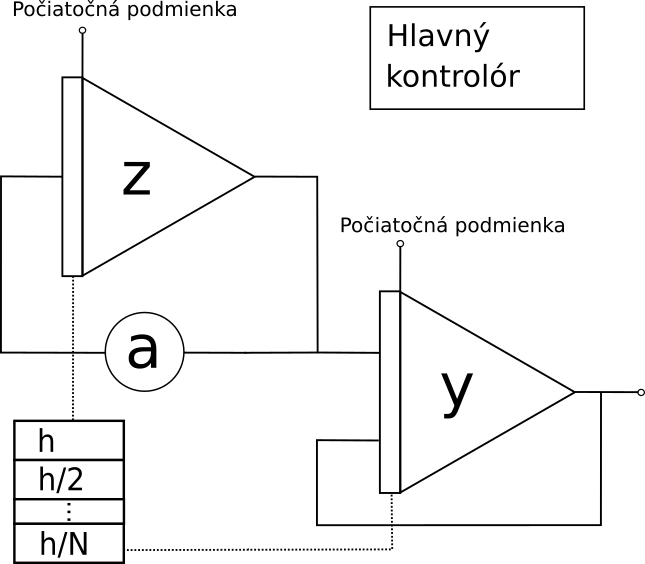
\includegraphics{obrazky/rovnica.png}}
\caption{Schéma zapojenia integrátorov}
\label{ppi_fp_sustava_impl}
\end{figure}


Ovládanie komponentov na prírpavku FitKit 2.0 je relizované cez terminál programu QDevKit. Komunikácia medzi MCU (Micro-Controller Unit) a FPGA prebiaha pomocou rozhrania \textit{SPI}. Jednotlivé hodnoty zadávané v termináli sú ukladané do pamäte a cez prevodník \textit{SPI\_ADC} privedené do registrov FPGA. Jednotlivé registre sú vybrané adresovým dekóderom. Po inicializácii komunikácie prebieha v nekonečnom cykle metódou pooling čítanie z riadiaceho registra a z registra výsledku. Hodnoty registrov sú vypisované v termináli v hexadecimálnej forme. Príkazom \textit{help} je možné zobraziť nápovedu ovládania integrátora. Príkazmi \textit{DATAY} a \textit{DATAV} je možné nahrať počiatočné podmienky do integrátorov \textit{y} a \textit{v}. Hondoty počiatočných podmienok je potrebné zadávať v hexadeximálnej forme s veľkými písmenami, keďže sa vykonáva prevod z textovej formy do číselnej, ktorá je následne uložená do registra. Krok metódy je stanovený na hodnotu \textit{0.1} a nie je možné meniť ho počas priebehu aplikácie. To je z dôvodu potreby predpočítania podielov kroku \textit{h}. Tie sú už predpočítané v sete registrov. Po zadaní počiatočných podmienok je možné spustiť výpočet pomocou príkazu \textit{START}. Tým sa nastaví povolovací signál \textit{EN} a začne sa výpočet. Následne je výsledok po jednom kroku zobrazený v termináli. Pre výpočet hodnoty v ďalšom kroku je potrebné zadať získaný výsledok ako počiatočnú podmienku násobiaceho integrátora \textit{y}. Novú počiatočnú podmienku je potrebné zadať aj pri jednovstupovom integrátore, tú však nepoznáme. Jednoduchým a užívateľsky príjemným riešením je automatické kopírovanie výsledných hodnôt v oboch integrátoroch z registrov \textit{RV} do registrov \textit{RD}. Preto bol pridaný signál \textit{RvToRd} do jednovstupového integrátora, ktorý umožní presun z jedného registra do druhého bez potreby nahrania počiatočnej podmienky príkazom \textit{DATAV}. Presun hodnoty v násobiacom integrátore je realizovaný na úrovni MCU, pomocou ktorého sa hodnota získaného výsledku uloží ako počiatočná podmienka. Celý tento postup je skrytý za jednoduchým príkazom \textit{NEXTY}.


\chapter{Analýza} \label{ANALYZA}
V tejto kapitole zanalyzujeme dosiahnuté výsledky. Analyzovať môžeme rôzne vlastnosti navrhnutého procesora a taktiež použitej Taylorovej rady. Najdôležitejšími vlastnosťami sú presnosť výsledku, časová náročnosť a priestorová zložitosť. V tejto analýze sa budeme zaoberať časovou zložitosťou numerických metód a ich presnosťou. Porovnáme Taylorovu radu s metódami nižších rádov, ako sú Eulerova metóda, metóda Runge-Kutta 2. rádu a metóda Runge-Kutta 4. rádu. Tieto metódy sú popísane v kapitole \ref{NUM_INTEGRACIA}.

V prvom rade vypočítame čas procesora, potrebný na výpočet sústavy rovníc \ref{rovnicasustava}. V každom takte sa procesor nachádza v nejakom stave. Z výpisu jednotlivých stavov kontrolórov tak môžeme vypočítať, koľko stavov je potrebných na výpočet pri použití rôzneho rádu metódy. Výsledný počet stavov potom uvádza, koľko taktov procesora je potrebných na výpočet. Z frekvencie procesora a z počtu taktov následne získame celkový čas výpočtu.

\bigskip
\begin{figure}[h]
\centering
\scalebox{0.4}{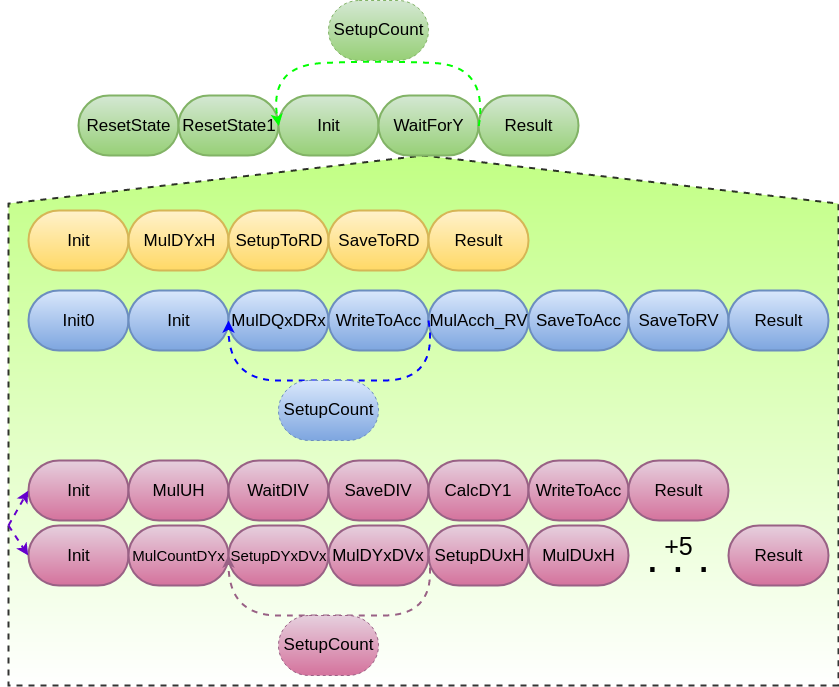
\includegraphics{obrazky/stavy.png}}
\caption{Stavy jednotlivých integrátorov.}
\label{stavyimg}
\end{figure}

Zobrazenie jednotlivých stavov kontrolórov je na obrázku \ref{stavyimg}. Jednotlivé bunky predstavujú stavy kontrolórov. Zelenou farbou je znázornený hlavný kontrolór, ktorý ovláda oba integrátory. Žltou farbou sú znázornené stavy jednovstupového integrátora a modrou farbou stavy násobiaceho integrátora. Hlavný kontrolór je v stave \textit{WeitForY} počas celého výpočtu integrátorov. Z tohto stavu prejde do ďalšieho stavu až po skončení výpočtu násobiaceho integrátora, keďže jeho výpočet trvá najdlhšie. Ak bol dosiahnutý maximálny rád metódy, hlavný kontrolór prejde do stavu \textit{Result}. V opačnom prípade výpočet pokračuje stavom \textit{SetupCount} a začne sa nový cyklus výpočtu. Počet taktov $ T_h $ hlavného kontrolóra, a teda celého výpočtu, môžeme vyjadriť vzťahom

\begin{eqnarray}
T_h & = & 2 + 1 + W + 2(N-1) + 1 \nonumber \\
T_h & = & 2 + W + 2N \, , \label{hkontrolerrovnica}
\end{eqnarray}

kde \textit{N} označuje počet cyklov výpočtu, čiže použitý rád Taylorovej metódy. Symbol $ W $ znamená počet stavov (taktov) v stave \textit{WaitForY}. Počet stavov xx sa rovná počtu stavov najdlhšie trvajúceho komponentu v sústave zapojenia. Označme potom \textit{W} ako $ W_{jv} $ pre jednovstupový integrátor, $ W_{nas} $ pre násobiaci integrátor a $ W_{div} $ pre deliaci integrátor.
Ak je v zapojení len jednovstupový integrátor, počet stavov je 5. Celkový čas výpočtu potom vyjadríme nasledovne:

\begin{eqnarray}
W_{jv} & = & 5N \nonumber \\ 
T_{jv} & = & (2 + W_{jv} + 2N)*t_{clk} \nonumber \\ 
T_{jv} & = & (2 + 5N + 2N)*t_{clk} \nonumber \\
T_{jv} & = & 2t_{clk} + 7t_{clk}N \, .
\end{eqnarray}

Symbol $ t_{clk} $ udáva čas periódy jedného taktu. Podobný výpočet vykonáme aj pre násobiaci a pre deliaci integrátor. Výpočet násobiaceho integrátora trvá 8 stavov a v každom ďalšom cykle je ich počet zvýšený o štyri. Z toho vyplýva, že

\begin{eqnarray}
W_{nas} & = & 6N + N(N+1) + \frac{N(N-1)}{2}  \nonumber \\
T_{nas} & = & \bigg(2 + W_{nas} + 2N\bigg)*t_{clk} \nonumber \\ 
T_{nas} & = & \bigg(2 + 6N + N(N+1) + \frac{N(N-1)}{2} + 2N\bigg)*t_{clk} \nonumber \\
T_{nas} & = & \bigg( 2 + 9N + N^2 + \dfrac{N(N-1)}{2}\bigg)*t_{clk} \, .
%T_{nas} & = & 1t_{clk} + 9t_{clk}N + 2t_{clk}N^2 \, .
\end{eqnarray}
\bigskip

Výpočet počtu krokov deliaceho integrátora je zložitejší. V prvom cykle sa vykonáva delenie a až pri výpočte ďalších členov Taylorovej rady sa násobia predchádzajúce členy \textit{DVx} a \textit{DUx} vo všetkých kombináciách medzi sebou. Výpočet stavov rozdelíme na počet stavov pre výpočet prvého člena a počet stavov pre výpočet ostatných členov Taylorovej rady. Rovnaké rozdelenie môžeme vidieť aj v konečnom automate deliaceho integrátora z obrázku \ref{stavyimg}. Počet stavov $ W_{div_1} $ pre prvý člen Taylorovej rady, počet stavov ostatných členov $ W_{div_x} $ a celkový počet krokov deliaceho integrátora vypočítame nasledovne:

\begin{eqnarray}
W_{div_1} & = & 6 + DIV \nonumber \\ 
W_{div_x} & = & 10(N-1) + N(N-1) + \frac{(N-1)(N-2)}{2} \nonumber \\ 
W_{div} & = & W_{div_1} + W_{div_x} \nonumber \\ 
W_{div} & = & 9N - 4 + DIV + N^2 + \frac{N^2-3N+2}{2} . \nonumber \\ 
\end{eqnarray}

Celkový čas výpočtu je potom 
\begin{eqnarray}
T_{div} & = & (2 + W_{div} + 2N)*t_{clk} \nonumber \\ 
T_{div} & = & \bigg(2 + 9N - 4 + DIV + N^2 + \frac{N^2-3N+2}{2} + 2N\bigg)*t_{clk} \nonumber \\
T_{div} & = & \bigg(DIV - 2 + 11N + N^2 + \frac{N^2-3N+2}{2}\bigg)*t_{clk} \, .
\end{eqnarray}

Zo vzťahov môžeme vidieť, že časová zložitosť výpočtu pri jednovstupovom integrátore je lineárna, pri násobiacom a pri deliacom integrátore je kvadratická. Časová zložitosť je znázornená na obrázku \ref{graf}. Je vidieť, že počet operácií deliaceho integrátora je len o niečo väčší než pri násobiacom integrátore. 

\begin{figure}[H]
\centering
\scalebox{0.6}{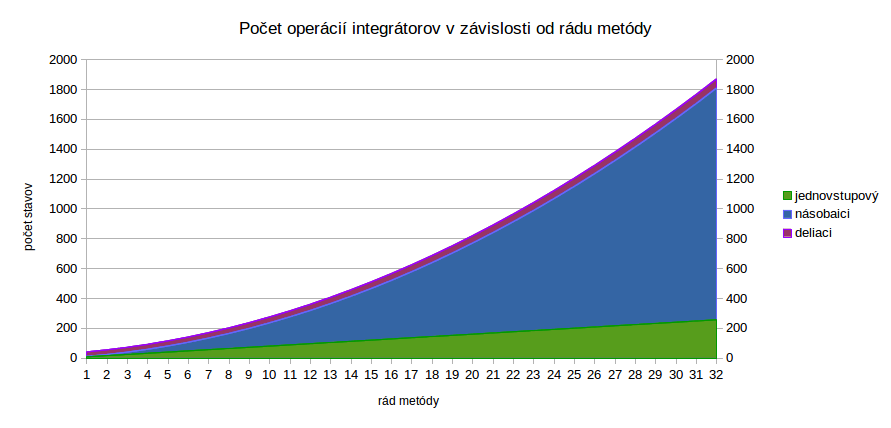
\includegraphics{obrazky/graf.png}}
\caption{Schéma zapojenia integrátorov}
\label{graf}
\end{figure}


\newpage
Ďalším analyzovaným kritériom je presnosť numerických metód. Na porovnanie presnosti potrebujeme poznať exaktné riešenie problému, ktorý riešime. Rovnica \eqref{rovnica} má exaktné riešenie nasledovné:

\begin{equation}
y' = e^{\frac{e^{at}}{a}} e^{-\frac{1}{a}} .
\end{equation}
\bigskip


Porovnanie jednotlivých metód je zobrazené v tabuľkách \ref{tableanalyza1} a \ref{tableanalyza2}. Porovnanie jednotlivých metód spočívalo v nájdení maximálneho kroku $ h_{max} $ každej z metód tak, aby rozdiel najvyšších členov metód v čase $ t_{max} $ bol čo najmenší. Chyba výpočtu Eulerovej metódy bola určená podľa vzťahu:
\begin{equation}
error = |y_{euler}(t_{max}) - y_{exact}(t_{max})|.
\end{equation}
\bigskip

Rovnaký postup výpočtu chyby bol použitý aj pri ostatných metódach. Výsledný počet operácií (stavov) výpočtu a chybu výsledku nájdeme v tabuľkách \ref{tableanalyza1} a \ref{tableanalyza2}. Tabuľka \ref{tableanalyza1} bola vytvorená s krokom \textit{h = 1.0} pre Taylorovu metódu 8. rádu. Maximálny čas bol stanovený na $ h_{max} = 1.0 $. Z tabuľky je vidieť, že najmenšiu chybu mala Eulerova metóda, čo je však spôsobené veľmi malým krokom, ktorý viedol k obrovskému množstvu operácií. Najlepší pomer medzi presnosťou a rýchlosťou majú metódy Runge-Kutta 4. rádu a Taylorova metóda. Chyba Taylorovej metódy je spôsobená hlavne pre veľkosť kroku.

%\scriptsize
%\catcode`\-=12
%\setlength\tabcolsep{1.5pt}
%\centering

% Please add the following required packages to your document preamble:
% \usepackage[table,xcdraw]{xcolor}
% If you use beamer only pass "xcolor=table" option, i.e. \documentclass[xcolor=table]{beamer}
\begin{table}[h]
\scriptsize
\catcode`\-=12
\setlength\tabcolsep{1.5pt}
\centering
\begin{tabular}{|l|r|r|r|r|r|r|r|}
\hline
\rowcolor[HTML]{34CDF9} 
\multicolumn{1}{|c|}{\cellcolor[HTML]{34CDF9}\textbf{metóda}} & \multicolumn{1}{c|}{\cellcolor[HTML]{34CDF9}\textbf{$h_{max}$}} & \multicolumn{1}{c|}{\cellcolor[HTML]{34CDF9}\textbf{\begin{tabular}[c]{@{}c@{}}hodnota\\ najvyššieho\\ člena\end{tabular}}} & \multicolumn{1}{c|}{\cellcolor[HTML]{34CDF9}\textbf{$t_{max}$}} & \multicolumn{1}{c|}{\cellcolor[HTML]{34CDF9}\textbf{výsledok}} & \multicolumn{1}{c|}{\cellcolor[HTML]{34CDF9}\textbf{error}} & \multicolumn{1}{c|}{\cellcolor[HTML]{34CDF9}\textbf{\begin{tabular}[c]{@{}c@{}}počet\\ krokov\\ {[}$t_{max}/h_{max}${]}\end{tabular}}} & \multicolumn{1}{c|}{\cellcolor[HTML]{34CDF9}\textbf{\begin{tabular}[c]{@{}c@{}}počet operácií\\ {[}$T*(t_{max}/h_{max})${]}\end{tabular}}} \\ \hline
\cellcolor[HTML]{DAE8FC}\textbf{Euler} & 0.00044 & 3.045E-04 & 1.00012 & 1.88165390491486 & 2.554E-05 & 2273 & 27 276 \\ \hline
\cellcolor[HTML]{DAE8FC}\textbf{R-K 2} & 0.03750 & -3.075E-04 & 1.01250 & 1.89048695564270 & 2.722E-04 & 27 & 675 \\ \hline
\cellcolor[HTML]{DAE8FC}\textbf{R-K 4.} & 0.35000 & 3.177E-04 & 1.05000 & 1.91570568084717 & 4.560E-05 & 3 & 123 \\ \hline
\cellcolor[HTML]{DAE8FC}\textbf{Taylor 8} & 1.00000 & -3.063E-04 & 1.00000 & 1.88219246082008 & 5.961E-04 & 1 & 60 \\ \hline
\end{tabular}
\caption{Porovnanie presnosti a rýchlosti numerických metód.}
\label{tableanalyza1}
\end{table}


V tabuľke \ref{tableanalyza1} bol numerický krok Taylorovej metódy 8. rádu znížený na polovciu, t. j. \textit{h = 0.5}. Eulerovu metódu už neberieme do úvahy, keďže počet operácií by bol priveľký. Pri porovnaní oboch tabuliek je vidieť, že pomer medzi presnosťou a rýchlosťou je najlepší pri Taylorovej metóde 8. rádu. Aby sme zachovali rovnakú presnosť Taylorovej metódy 8. rádu, v metóde Runge-Kutta 4. rádu je potrebné zvoliť dostatočne malý krok, avšak počet operácií sa tým niekoľkokrát zvýši. V tomto konkrétnom príklade sa počet operácií zvýšil štvornásobne. Ďalej si môžeme všimnúť, že metóda si udržuje presnosť vzhľadom na hodnotu posledného člena metódy. 

% Please add the following required packages to your document preamble:
% \usepackage[table,xcdraw]{xcolor}
% If you use beamer only pass "xcolor=table" option, i.e. \documentclass[xcolor=table]{beamer}
\begin{table}[h]
\scriptsize
\catcode`\-=12
\setlength\tabcolsep{1.5pt}
\centering
\begin{tabular}{|l|r|r|r|r|r|r|r|}
\hline
\rowcolor[HTML]{34CDF9} 
\multicolumn{1}{|c|}{\cellcolor[HTML]{34CDF9}\textbf{metóda}} & \multicolumn{1}{c|}{\cellcolor[HTML]{34CDF9}\textbf{$h_{max}$}} & \multicolumn{1}{c|}{\cellcolor[HTML]{34CDF9}\textbf{\begin{tabular}[c]{@{}c@{}}hodnota\\ najvyššieho\\ člena\end{tabular}}} & \multicolumn{1}{c|}{\cellcolor[HTML]{34CDF9}\textbf{$t_{max}$}} & \multicolumn{1}{c|}{\cellcolor[HTML]{34CDF9}\textbf{výsledok}} & \multicolumn{1}{c|}{\cellcolor[HTML]{34CDF9}\textbf{error}} & \multicolumn{1}{c|}{\cellcolor[HTML]{34CDF9}\textbf{\begin{tabular}[c]{@{}c@{}}počet\\ krokov\\ {[}$t_{max}/h_{max}${]}\end{tabular}}} & \multicolumn{1}{c|}{\cellcolor[HTML]{34CDF9}\textbf{\begin{tabular}[c]{@{}c@{}}počet operácií\\ {[}$T*(t_{max}/h_{max})${]}\end{tabular}}} \\ \hline
\cellcolor[HTML]{DAE8FC}\textbf{R-K 2} & 0.00234 & -1.198E-06 & 0.99918 & 1.88102829456329 & 2.377E-06 & 427 & 10 675 \\ \hline
\cellcolor[HTML]{DAE8FC}\textbf{R-K 4.} & 0.08580 & 1.197E-06 & 1.02960 & 1.90189445018768 & 4.788E-07 & 12 & 492 \\ \hline
\cellcolor[HTML]{DAE8FC}\textbf{Taylor 8} & 0.50000 & 1.196E-06 & 1.00000 & 1.88159812241793 & 1.735E-06 & 1 & 120 \\ \hline
\end{tabular}
\caption{Porovnanie presnosti a rýchlosti numerických metód.}
\label{tableanalyza2}
\end{table}

Nasledujúce obrázky \ref{modelsim1} a \ref{modelsim2} zachytávajú simuláciu Taylorovej rady 8. rádu v programe ModelSim na výpočet hodnôt v predchádzajúcich tabuľkách. Na obrázkoch je červenou farbou zvýraznený register výsledku \textit{RV} násobiaceho integrátora. Stavy označené zelenou farbou patria hlavnému kontrolóru. Žltou farbou je označený aktuálny stav jednovstupového integrátora, modrou farbou sú označené stavy násobiaceho integrátora. Hodnota v registri je zobrazená hexadecimálne a zodpovedá decimálnej hodnote uvedenej ako výsledok v predchádzajúcich tabuľkách. 

\begin{figure}[H]
\centering
\scalebox{0.6}{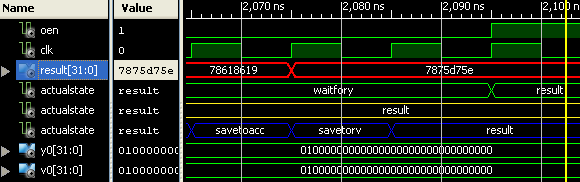
\includegraphics{obrazky/modelsim81.png}}
\caption{Simulácia sústavy rovníc \ref{rovnicasustava} Taylorovou radou 8. rádu s $ h = 1 $ a $ h_{max} = 1 $.}
\label{modelsim1}
\end{figure}

\begin{figure}[H]
\centering
\scalebox{0.6}{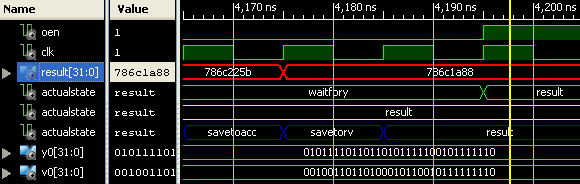
\includegraphics{obrazky/modelsim82.png}}
\caption{Simulácia sústavy rovníc \ref{rovnicasustava} Taylorovou radou 8. rádu s $ h = 0.5 $ a $ h_{max} = 1 $.}
\label{modelsim2}
\end{figure}


\chapter{Záver}
V~tejto práci sme sa zaoberali riešením počiatočných úloh s využitím numerickej integrácie pomocou modernej metódy Taylorovej rady. Úpravou jej členov sme získali potrebné rovnice, z~ktorých boli vytvorené jednotlivé návrhy integrátorov. Navrhli sme paralelné integrátory v pevnej a v pohyblivej rádovej čiarke s operáciou násobenia a delenia. Ďalej sme rozšírili návrhy týchto paralelných integrátorov tak, aby bol nimi možný výpočet ako samostatného komponentu, tak aj komponentu zapojeného do sústavy. Následne sme navrhnuté integrátory popísali vo VHDL a otestovali ich pomocou \textit{testbanchu} v simulačnom nástroji \textit{ModelSim}. Takto pripravené integrátory sme potom implementovali v FPGA, kde bola otestovaná ich funkčnosť. Implementovaný bol aj jednovstupový integrátor navrhnutý v práci \cite{OpalkaDP}. Tento paralelný integrátor bol taktiež implementovaný v prevedení pevnej a pohyblivej rádovej čiarky. Na ovládanie integrátorov sme použili terminál programu \textit{QDevKit}. Zjednodušili sme ovládanie integrátorov pridaním príkazu $ nexty $, ktorý umožňuje výpočet ďalšieho kroku riešenej rovnice bez opätovného zadávania počiatočných podmienok.

Takto implementované integrátory môžu byť použité pri výučbe hardvérových predmetov a predmetov venujúcich sa numerickej integrácii. V poslednej kapitole sme sa venovali časovej analýze navrhnutých integrátorov. Ďalej sme porovnali presnosť Taylorovej metódy s Eulerovou metódou a s metódami Runge-Kutta 2. a 4. rádu. Z analýzy sme zistili, že najlepší pomer medzi presnosťou a rýchlosťou z porovnávaných metód má Taylorova rada 8. rádu.

Ďalším pokračovaním práce môže byť návrh a implementácia kontrolóra pre rozsiahlejšie rovnice s použitím väčšieho programovateľného hradlového poľa. xx Vytvorenie prepojovacej siete integrátorov s dynamickou konfiguráciou prepojení pre riešenie rôznych sústav diferenciálnych rovníc.

%=========================================================================
